%%%%%%%%%%%%%%%%%%%%%%%%%%%%%%%%%%%%%%%%%%%%%%%%%%%%%%
%%%%%%%%%%%%%%%%%%%%%%%%%%%%%%%%%%%%%%%%%%%%%%%%%%%%%%
%%%%%%%%%%%%%%%%%%%%%%%%%%%%%%%%%%%%%%%%%%%%%%%%%%%%%%
\subsection{Partially unblinded data}


\begin{itemize}
    \item year 2015+2016
    \item year 2017
    \item year 2018
    \item Run 2: sum of all years.
    \item Combined Run 2: stitch up three datasets in the range of $0\to 6\pi$. The 2015+2016 dataset is in the $0\to 2\pi$ range, the 2017 dataset is in the $2pi\to 4\pi$ range, and 2018 dataset is in the $4pi\to 6\pi$ range.
\end{itemize}


\subsubsection{Fit results}

\begin{figure}[ht]
\centering
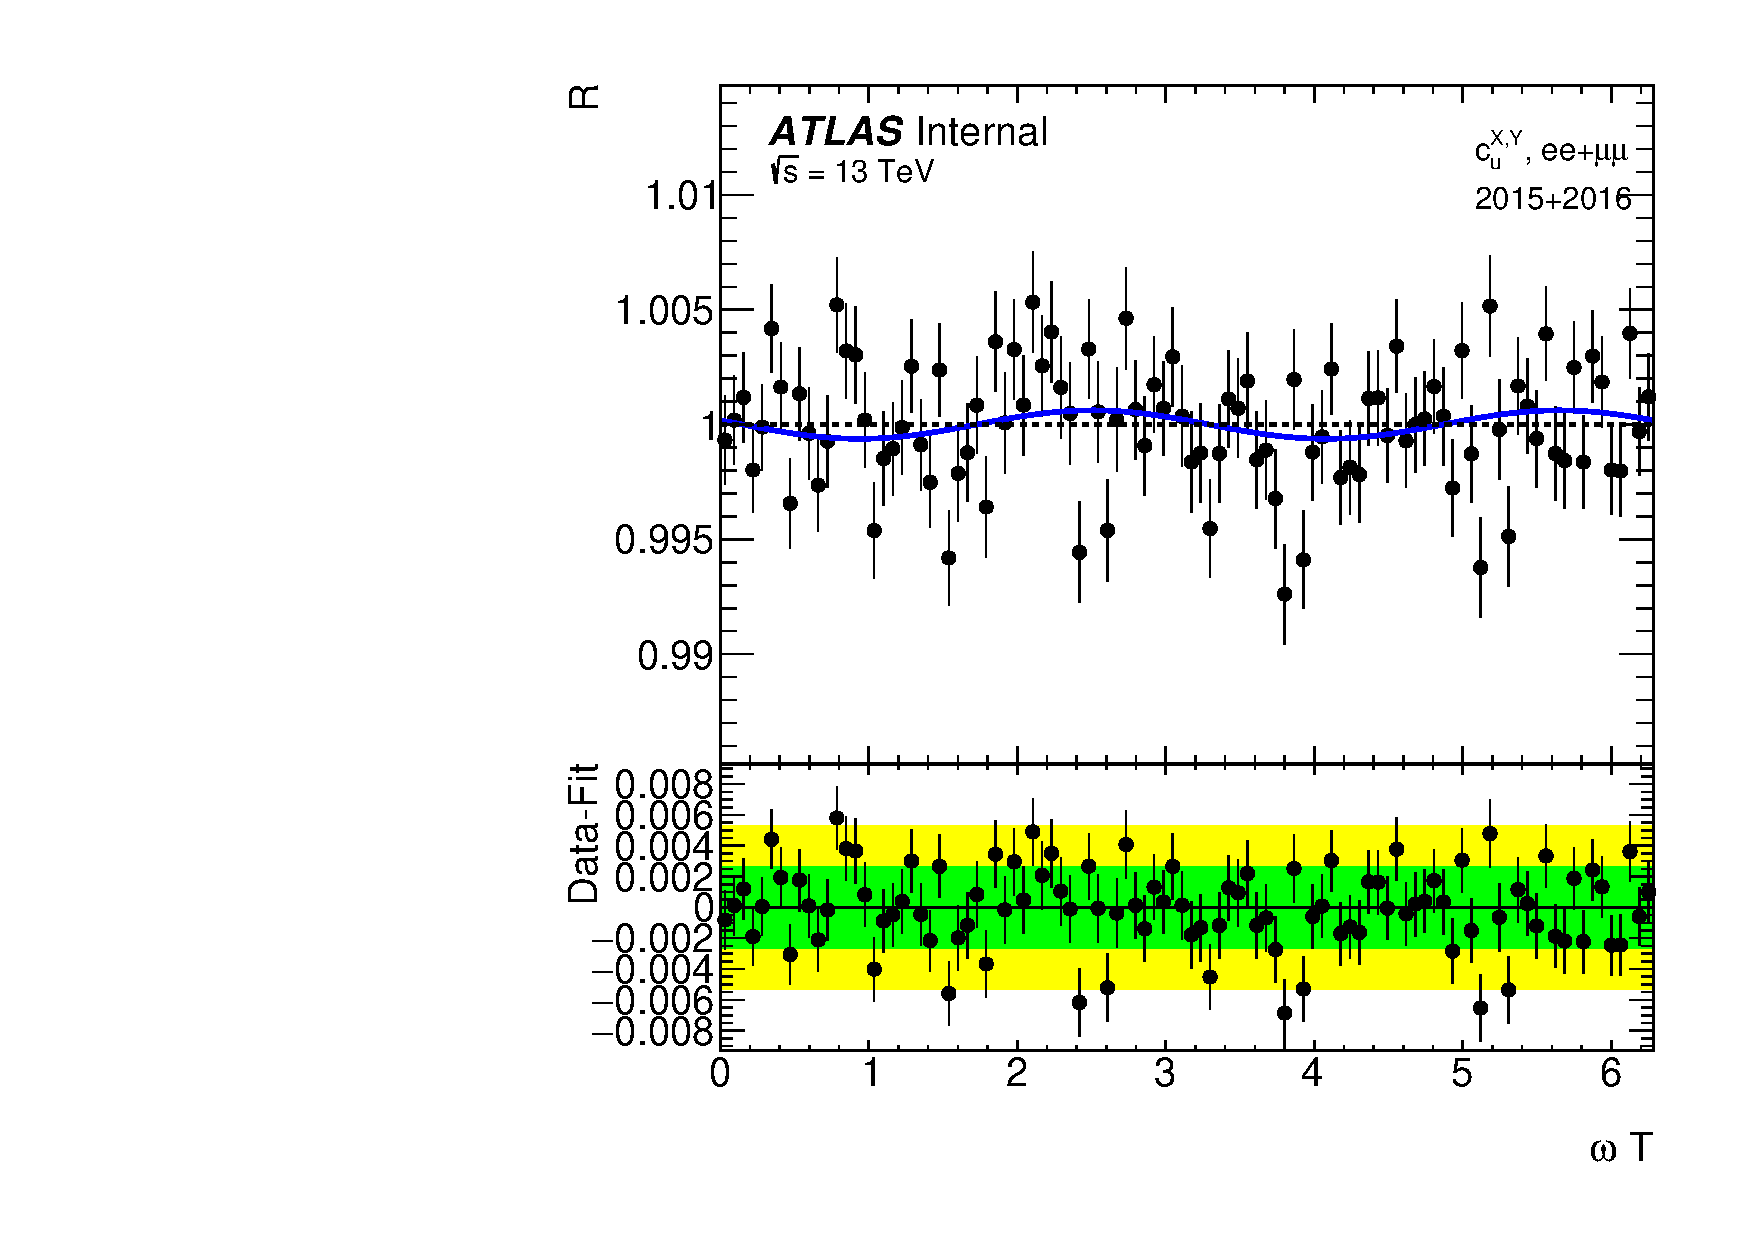
\includegraphics[width=0.45\textwidth]{figs/partially_unblinded_results/fit_results_residual_12func_ll_c[u,X,Y]_toy10_data15p16}
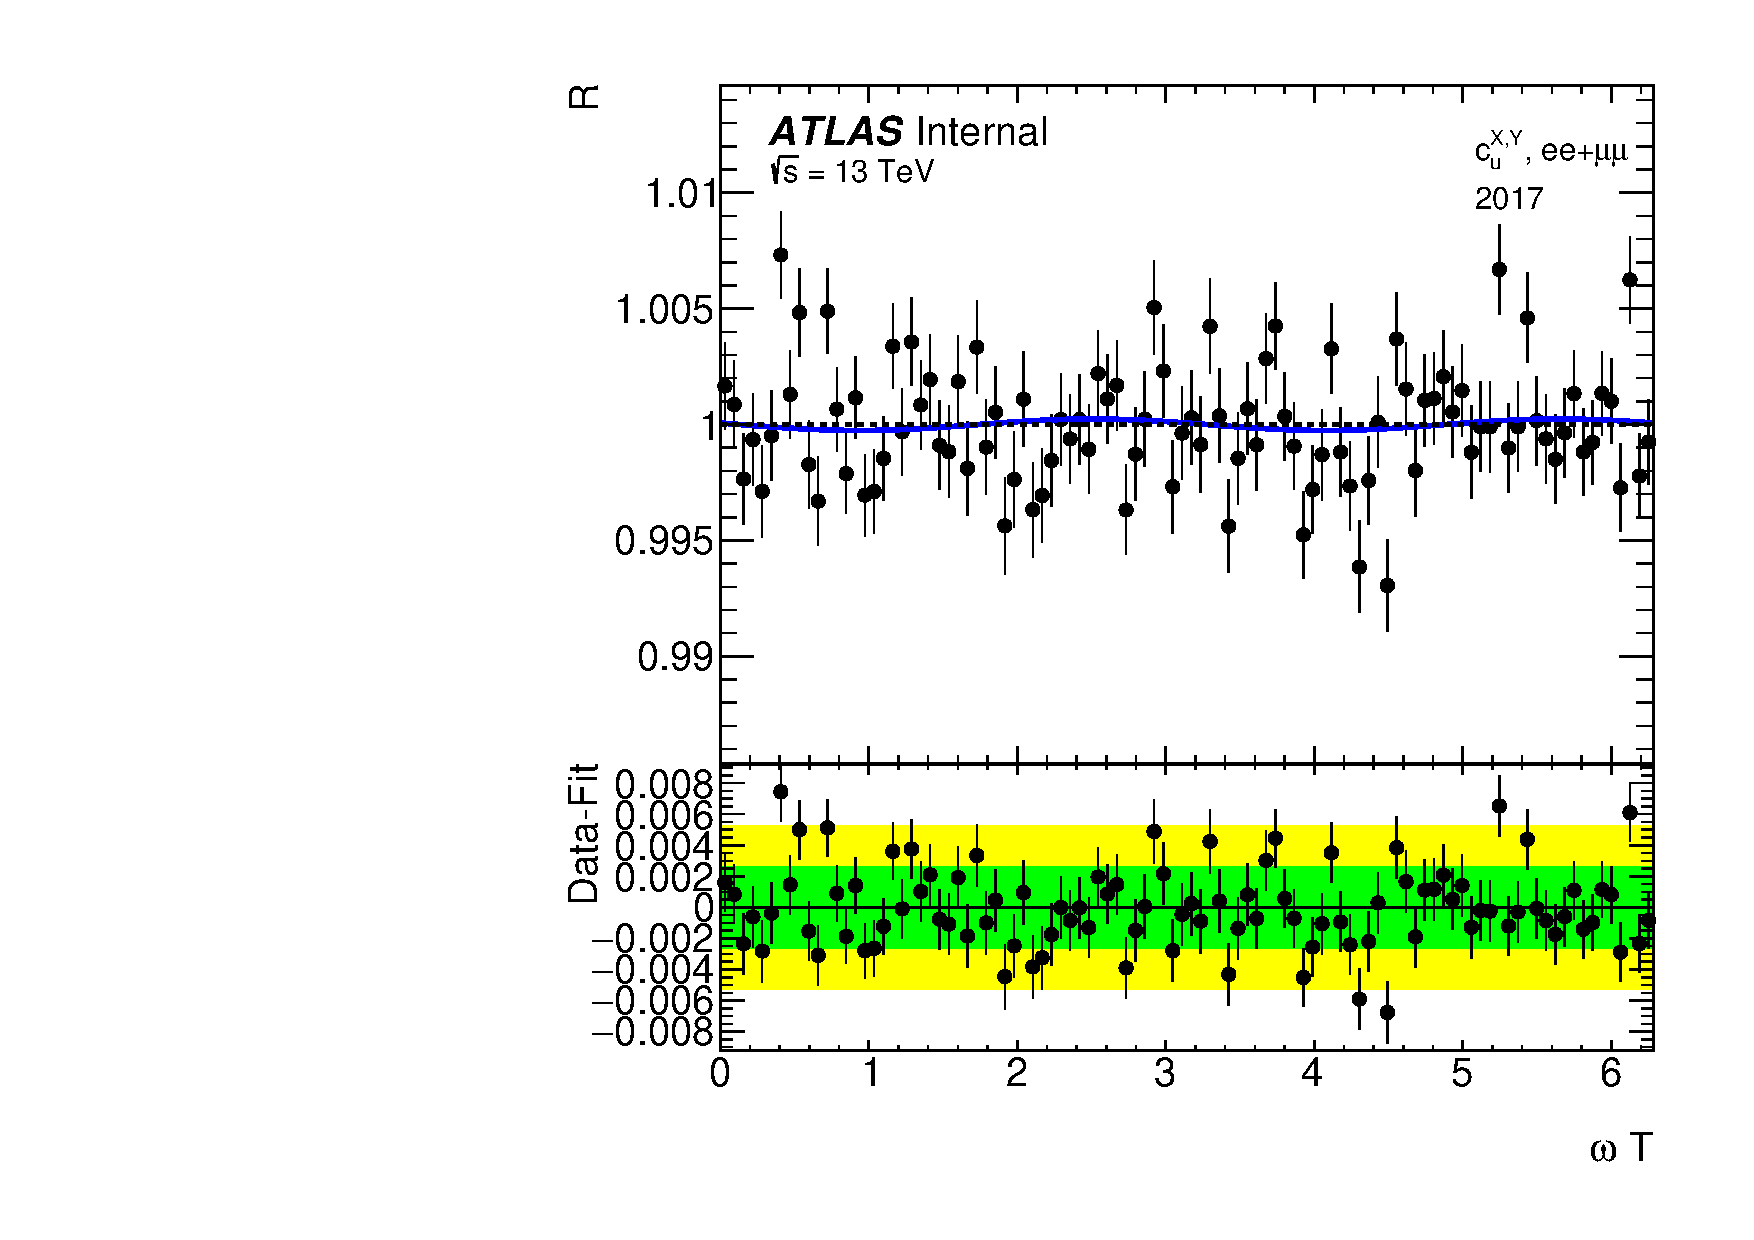
\includegraphics[width=0.45\textwidth]{figs/partially_unblinded_results/fit_results_residual_12func_ll_c[u,X,Y]_toy10_data17}\\
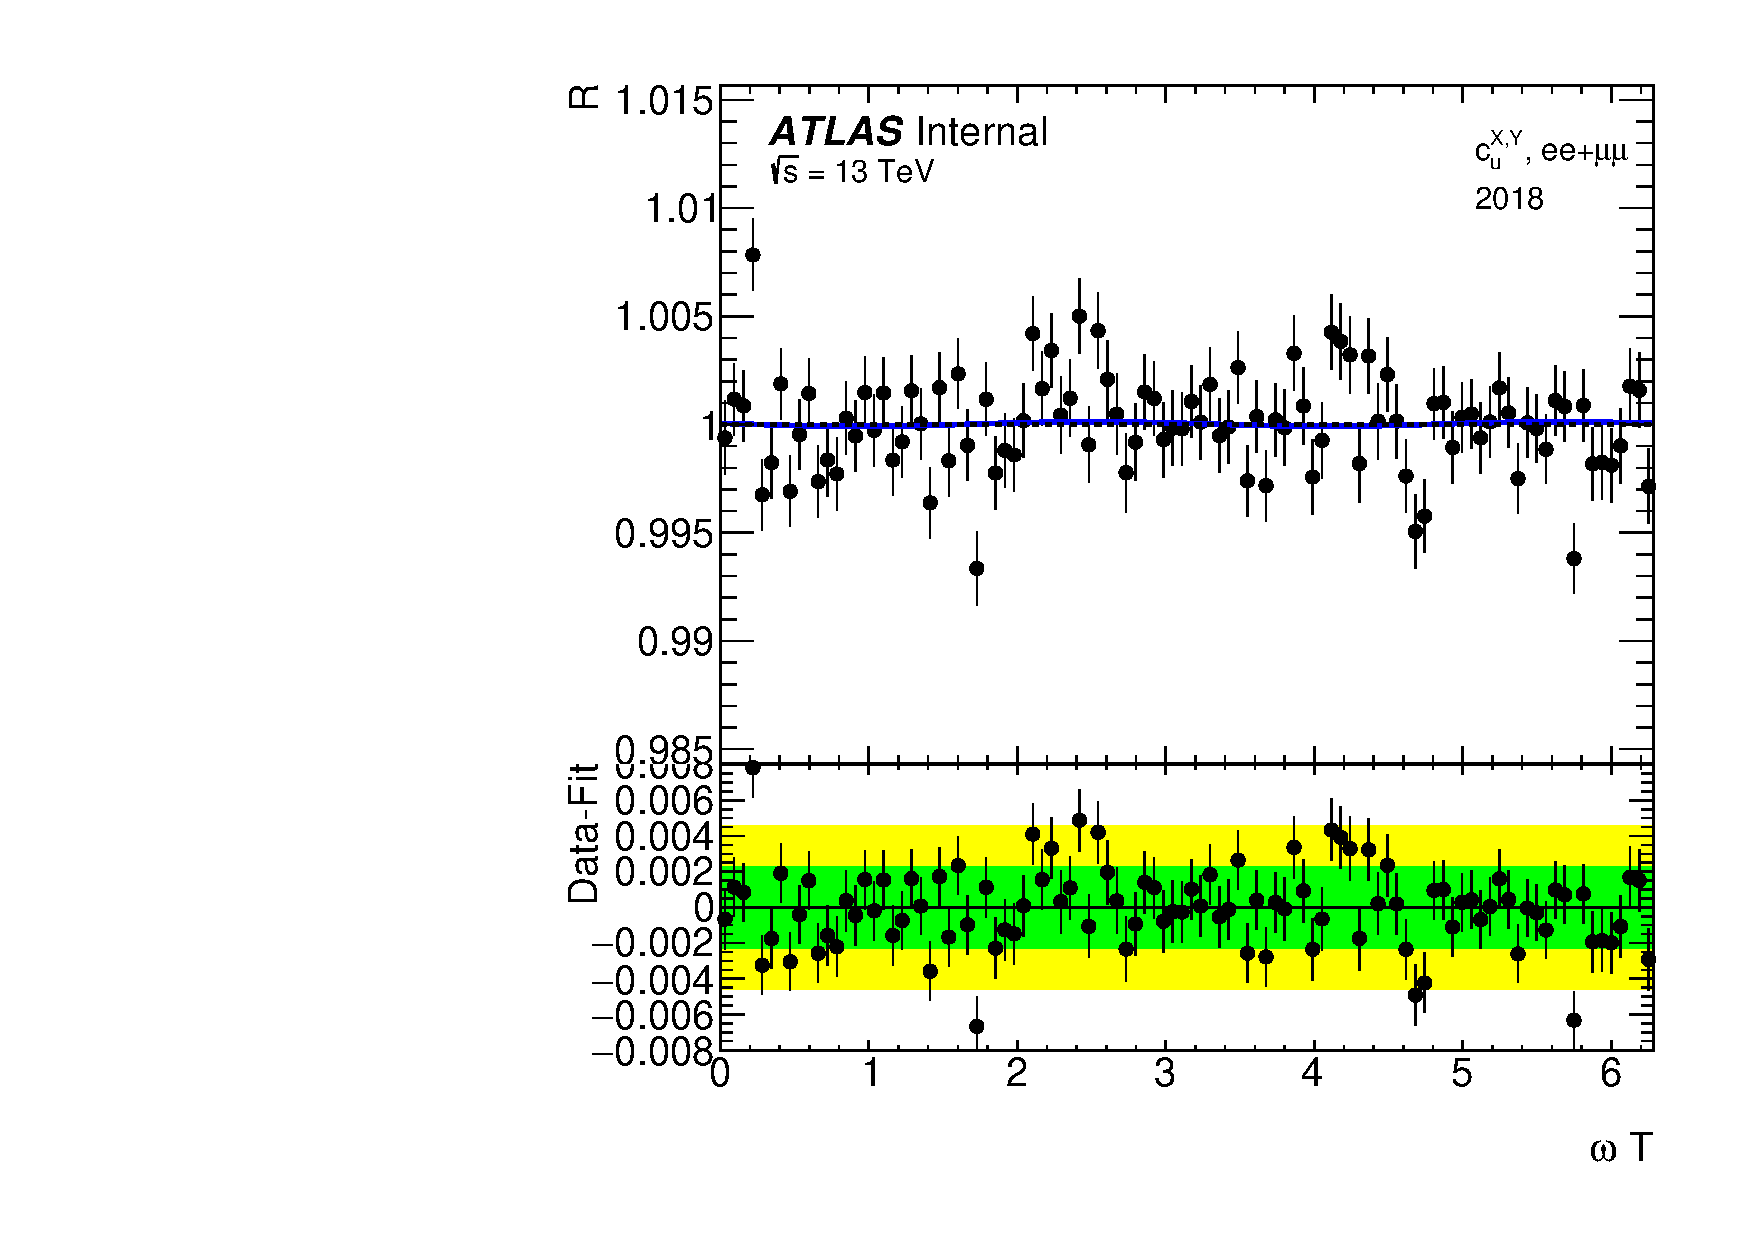
\includegraphics[width=0.45\textwidth]{figs/partially_unblinded_results/fit_results_residual_12func_ll_c[u,X,Y]_toy10_data18}
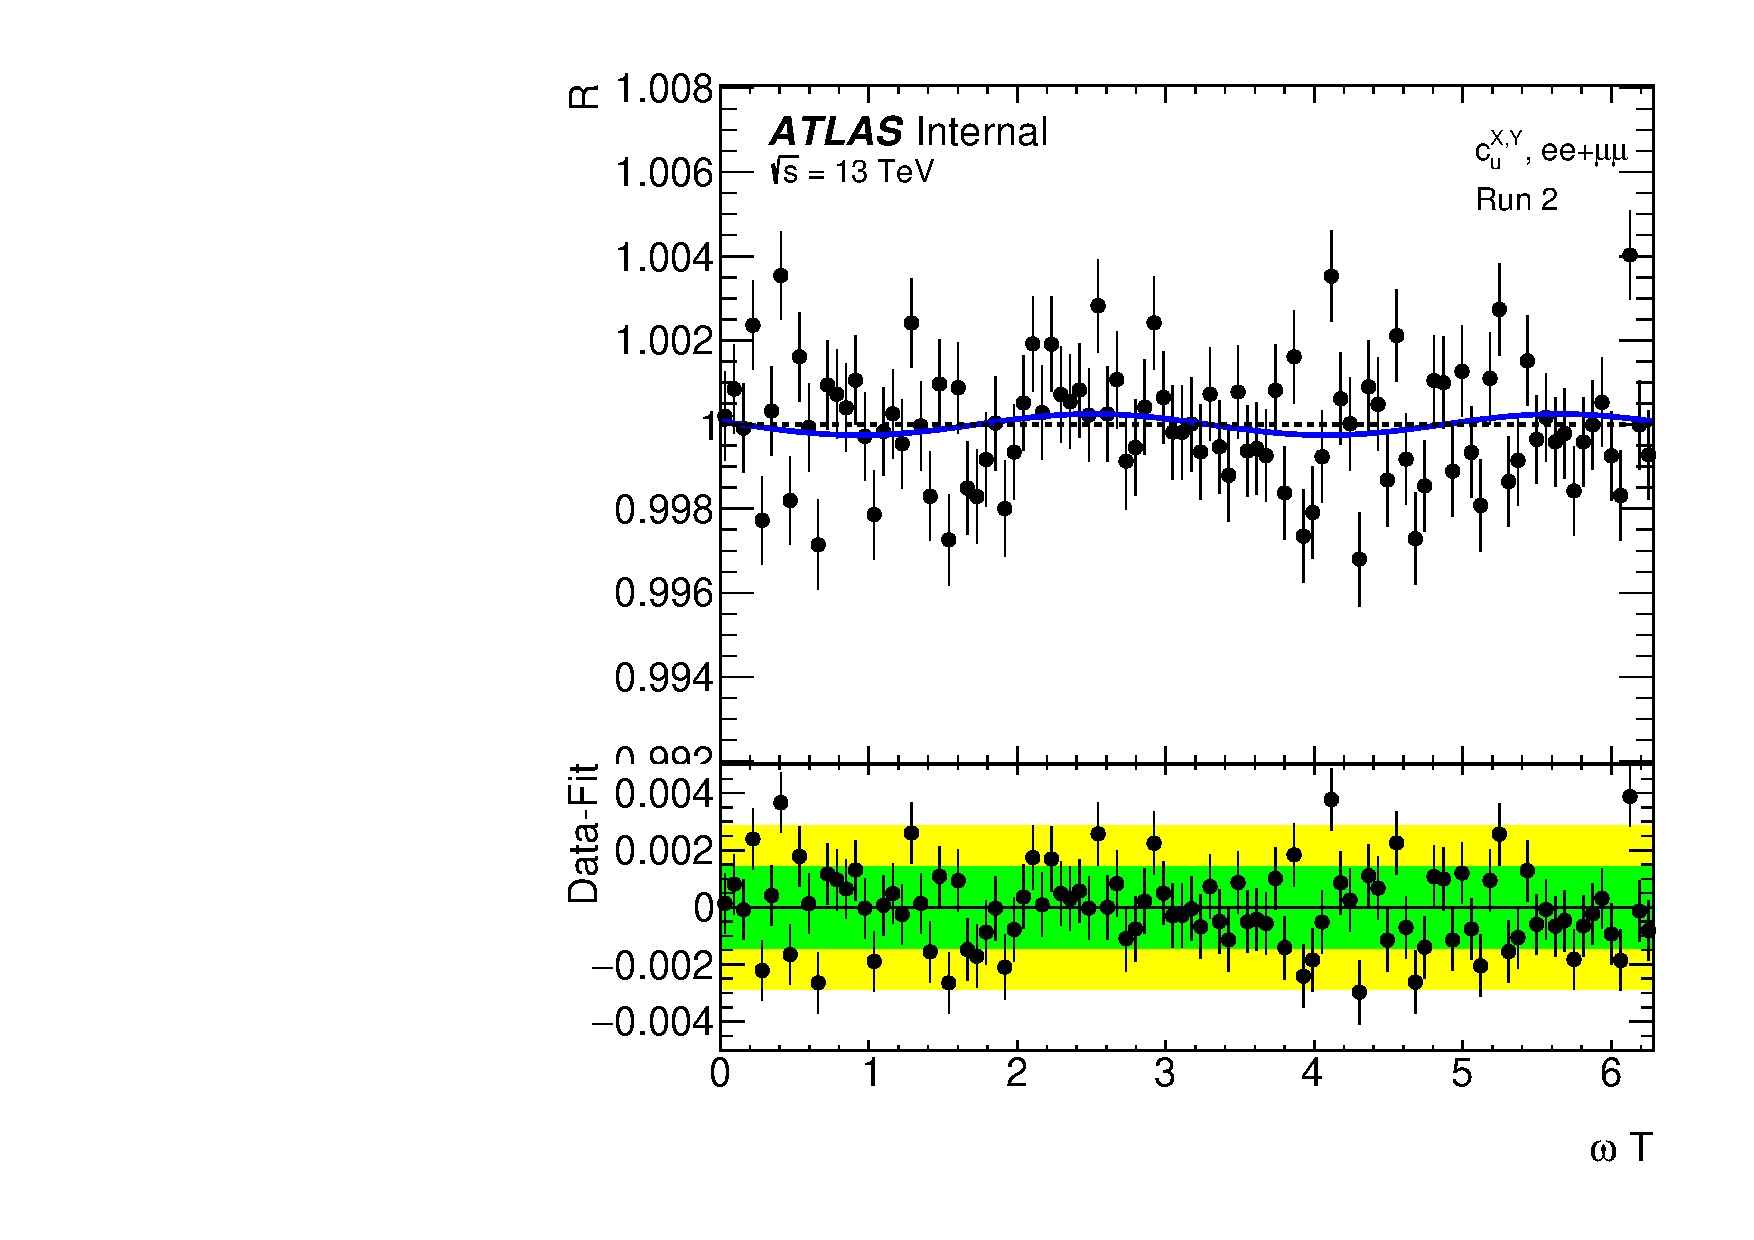
\includegraphics[width=0.45\textwidth]{figs/partially_unblinded_results/fit_results_residual_12func_ll_c[u,X,Y]_toy10_full}
\caption{One of the scrambled datasets VS $c_{u}^{X,Y}$ model. The black dots are the scrambled data, and the blue lines are the fitted model. The 2015+2016 dataset(top left), the 2017 dataset (top right), the 2018 dataset(bottom left), and the Run 2 dataset (bottom right). The Run 2 dataset is the sum of all year's data. The bottom panel of the plots is the residual (data-model). The green and yellow bands correspond to one and two sigma uncertainty bands.}
\label{fig:real_data_scrambled_oneDataset_Run2}
\end{figure}

\begin{figure}[ht]
\centering
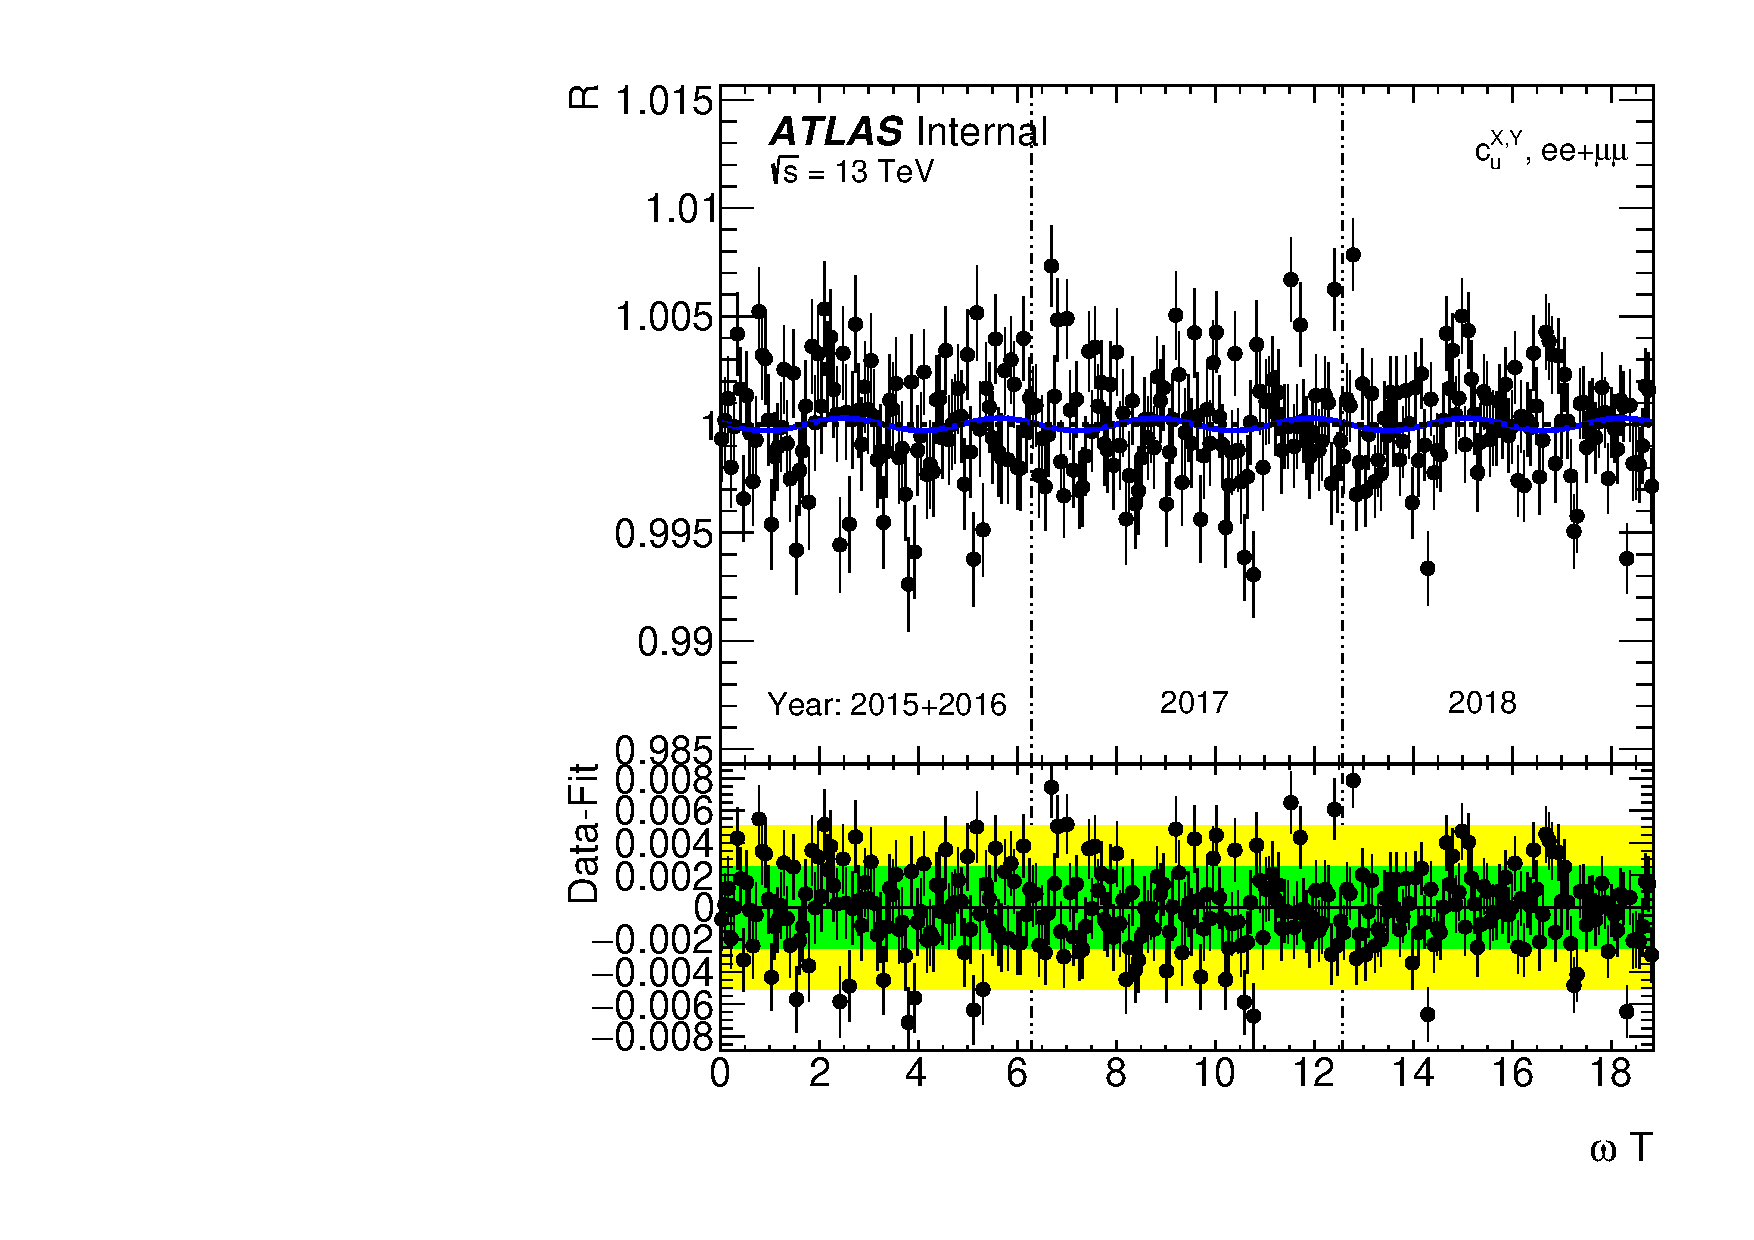
\includegraphics[width=0.6\textwidth]{figs/partially_unblinded_results/fit_results_residual_12func_ll_c[u,X,Y]_toy10_Combined}
\caption{The Run 2 combined dataset (ne of the scrambled datasets) VS $c_{u}^{X,Y}$ model. The black dots are the scrambled data, and the blue lines are the fitted model. The bottom panel of the plots is the residual (data-model). The green and yellow bands correspond to one and two sigma uncertainty bands.}
\label{fig:real_data_scrambled_oneDataset_combined}
\end{figure}





\begin{figure}[ht]
\centering
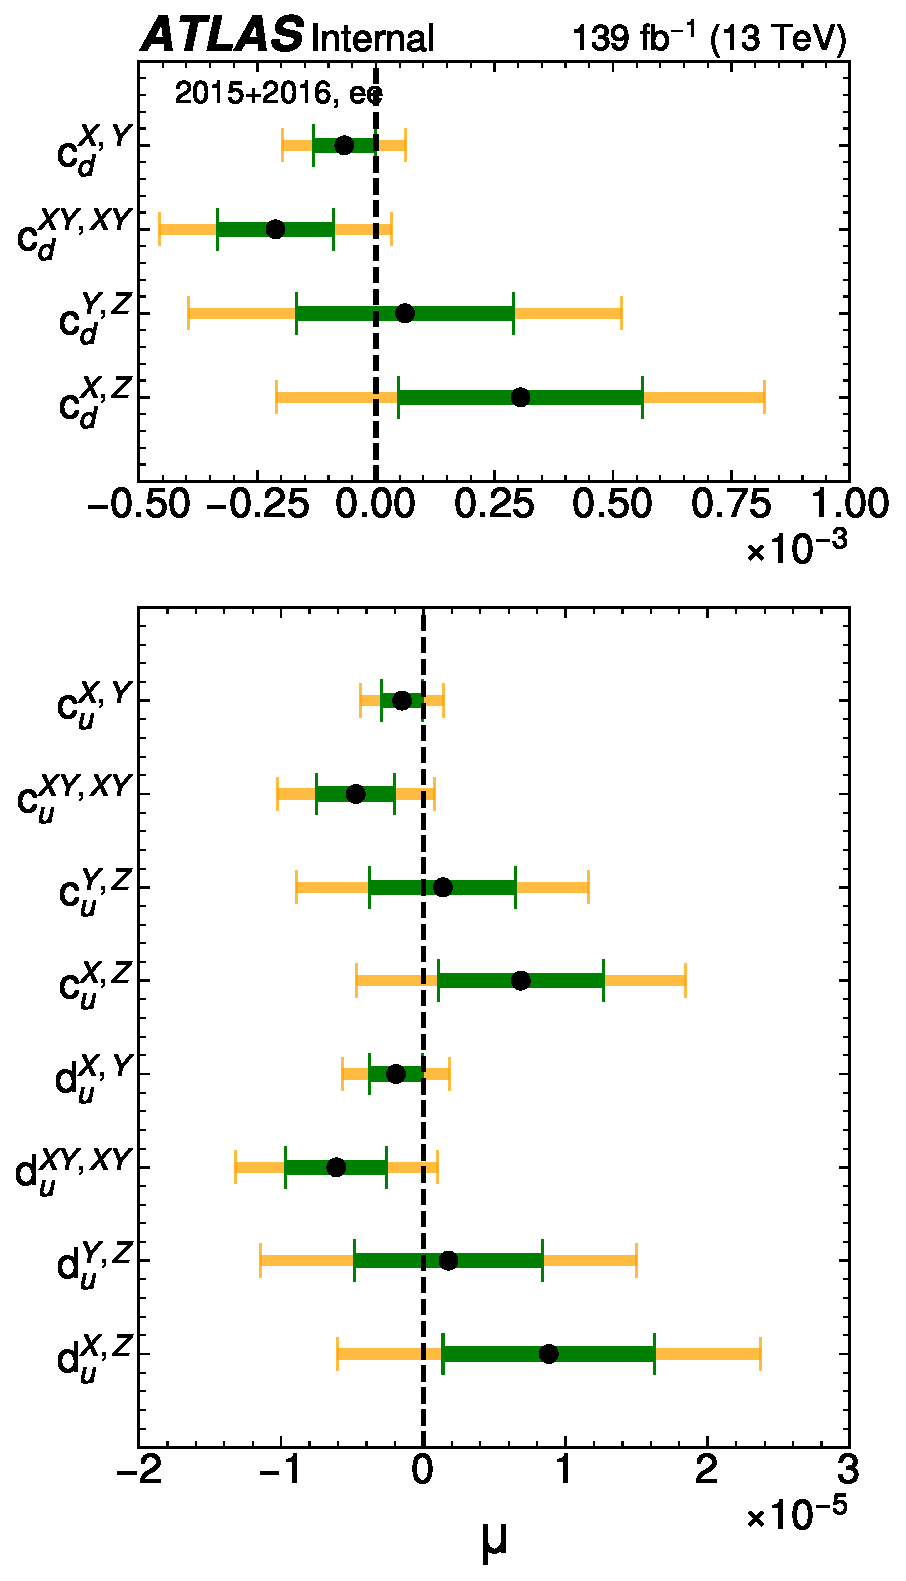
\includegraphics[width=0.30\textwidth]{figs/partially_unblinded_results/SigFit_summary_AllSamples_data15p16_ee.pdf}
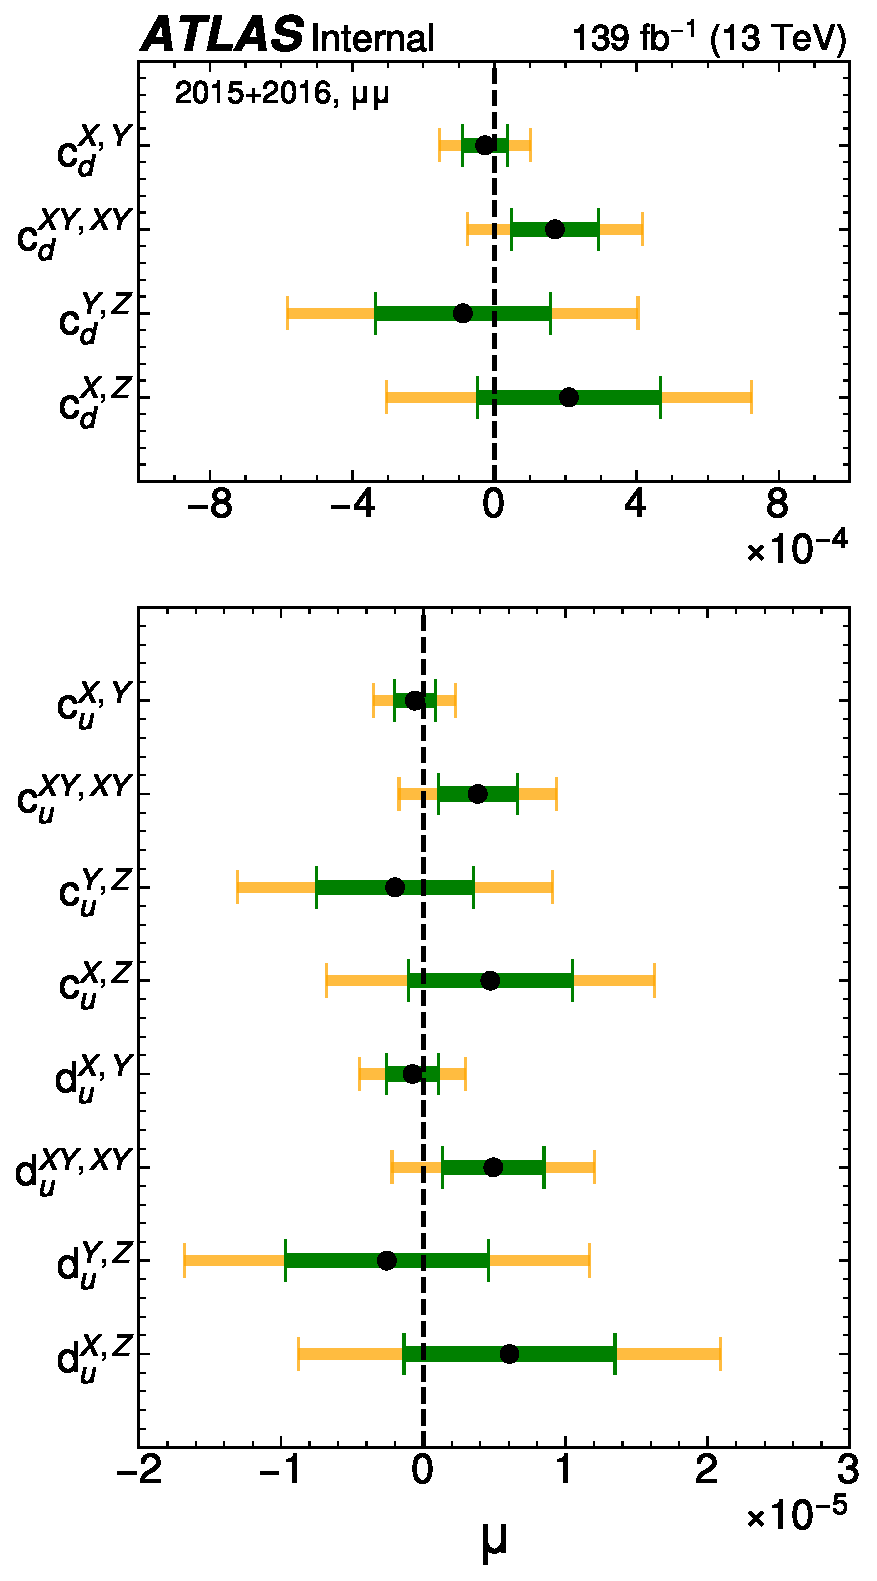
\includegraphics[width=0.30\textwidth]{figs/partially_unblinded_results/SigFit_summary_AllSamples_data15p16_uu.pdf}
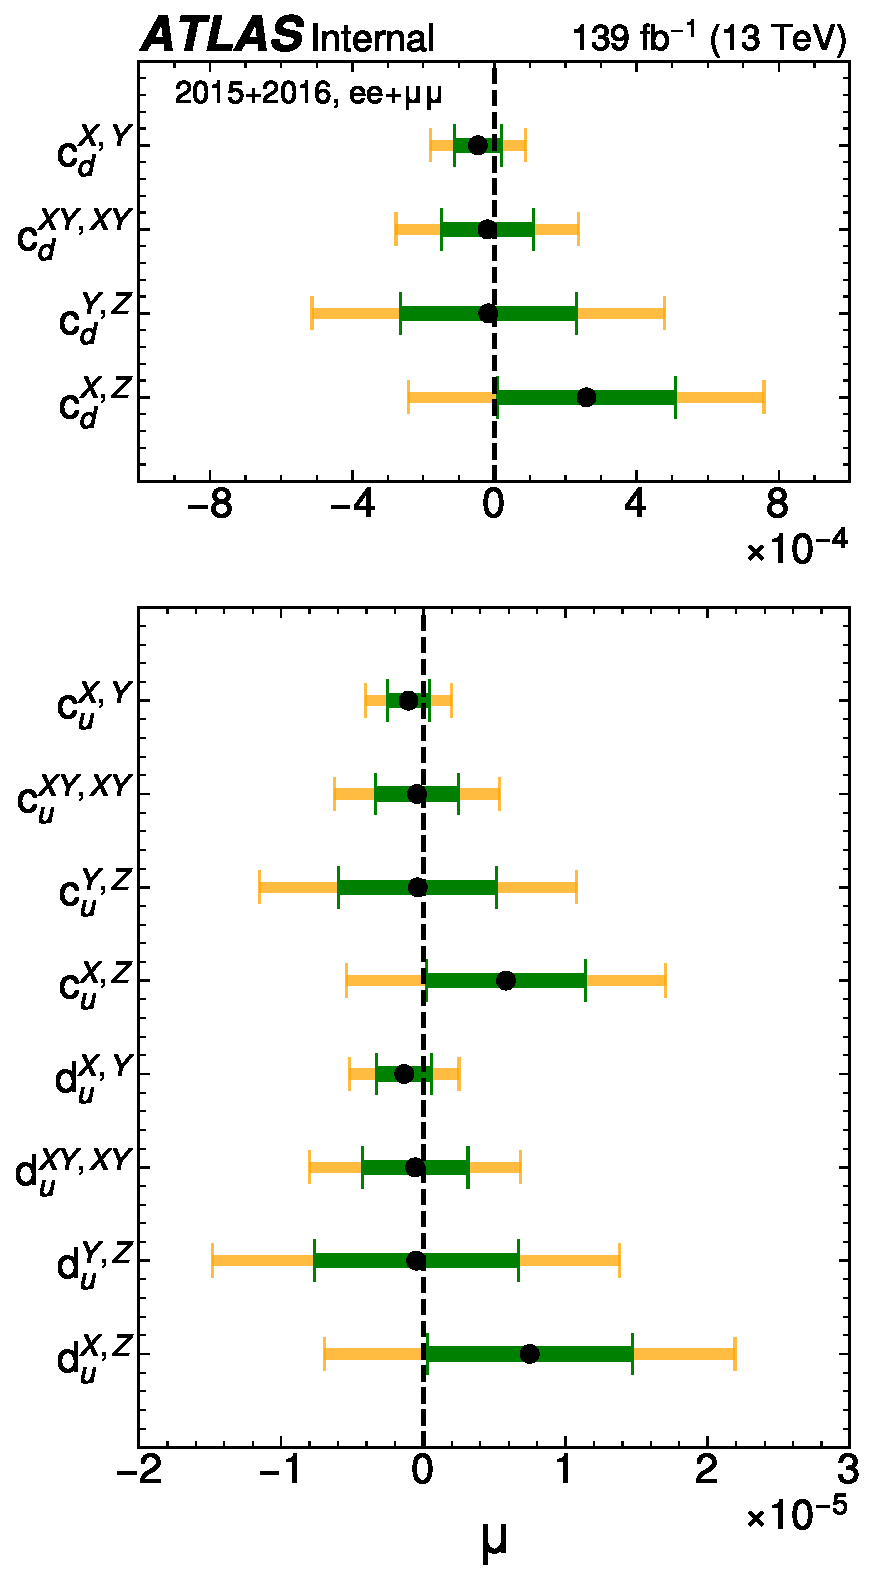
\includegraphics[width=0.30\textwidth]{figs/partially_unblinded_results/SigFit_summary_AllSamples_data15p16_ll.pdf}
\caption{Scrambled datasets collected in 2015 and 2016. Plots show average and one (two) standard deviation of 1000 fit results. The black dots are the average values of 1000 fit results, and the green (yellow) band is the corresponding one (two) sigma band. The $ee$ channel is in the left, the $\mu\mu$ channel is in the middle, and the $ee+\mu\mu$ is in the right.}
\label{fig:real_data_scrambled_summary_data15p16}
\end{figure}


\begin{figure}[ht]
\centering
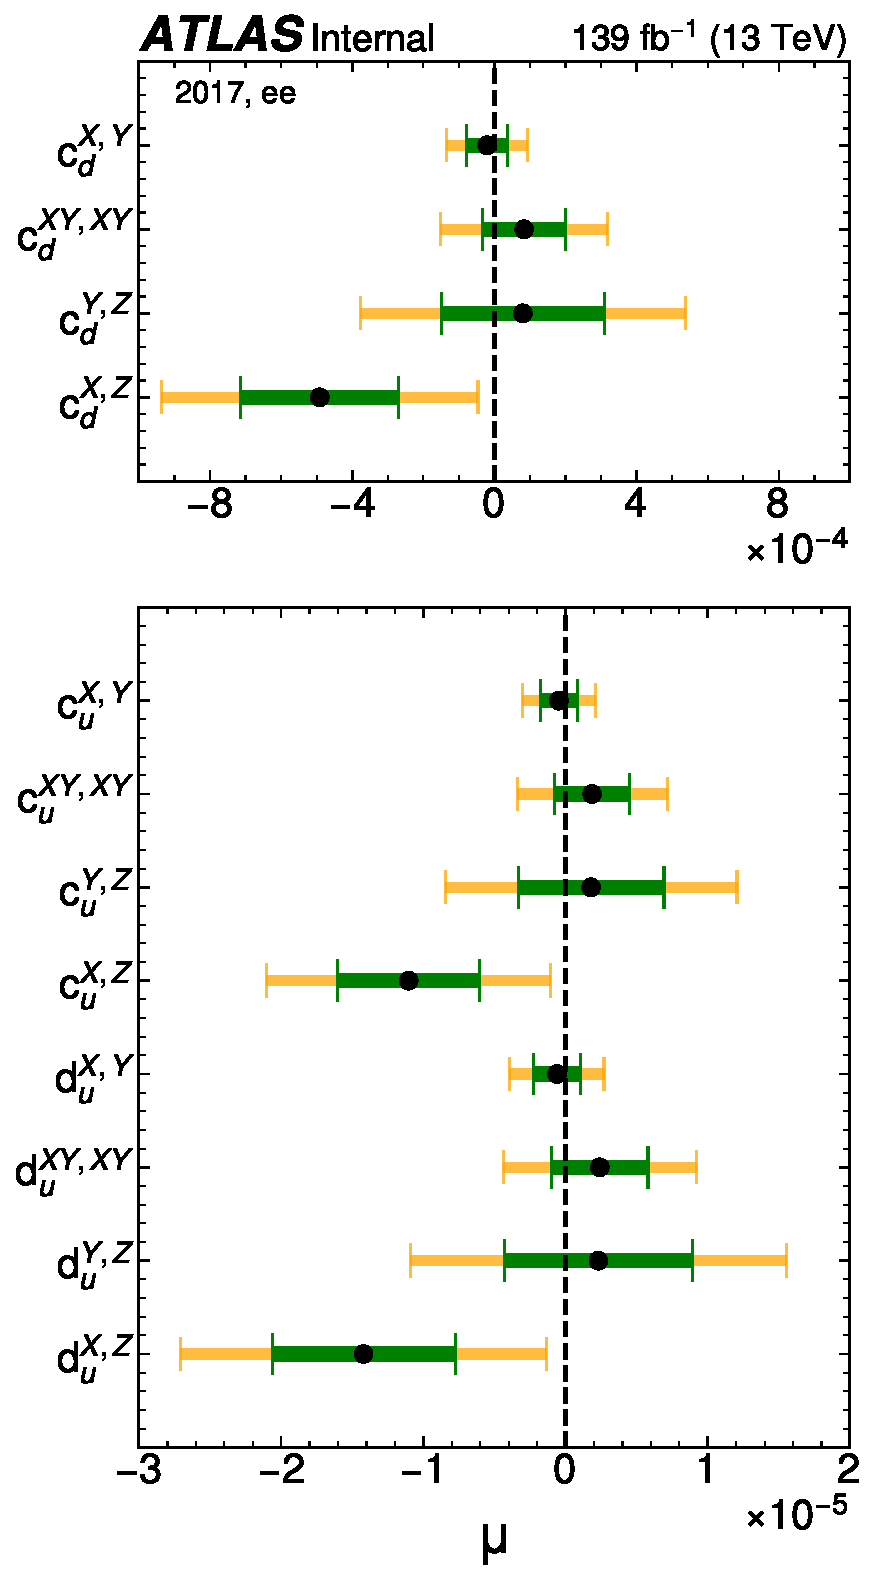
\includegraphics[width=0.30\textwidth]{figs/partially_unblinded_results/SigFit_summary_AllSamples_data17_ee.pdf}
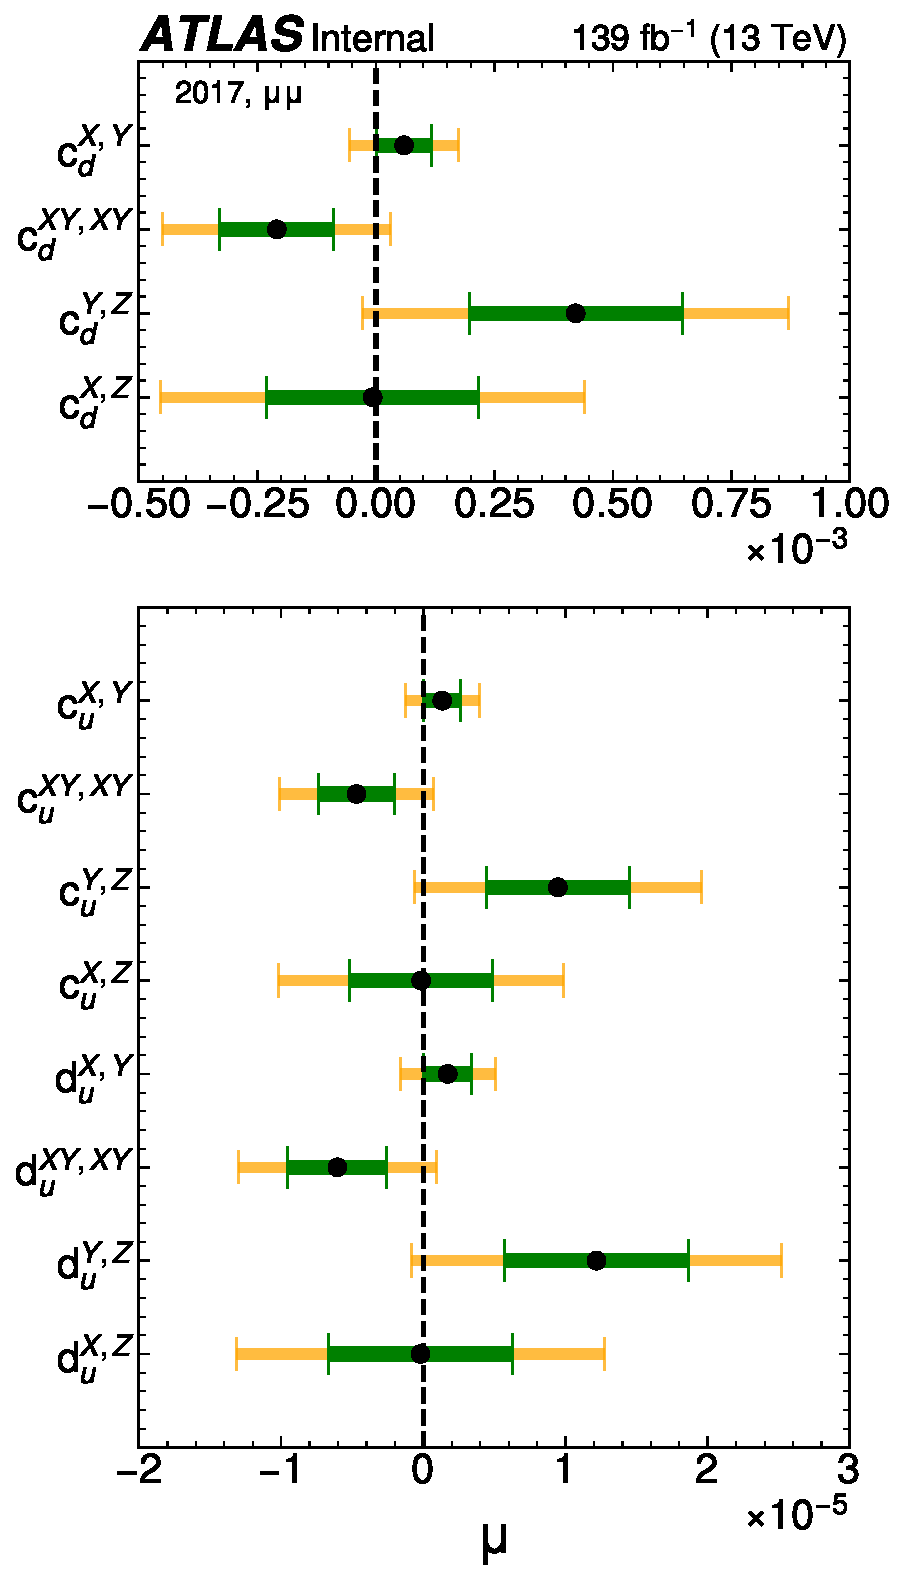
\includegraphics[width=0.30\textwidth]{figs/partially_unblinded_results/SigFit_summary_AllSamples_data17_uu.pdf}
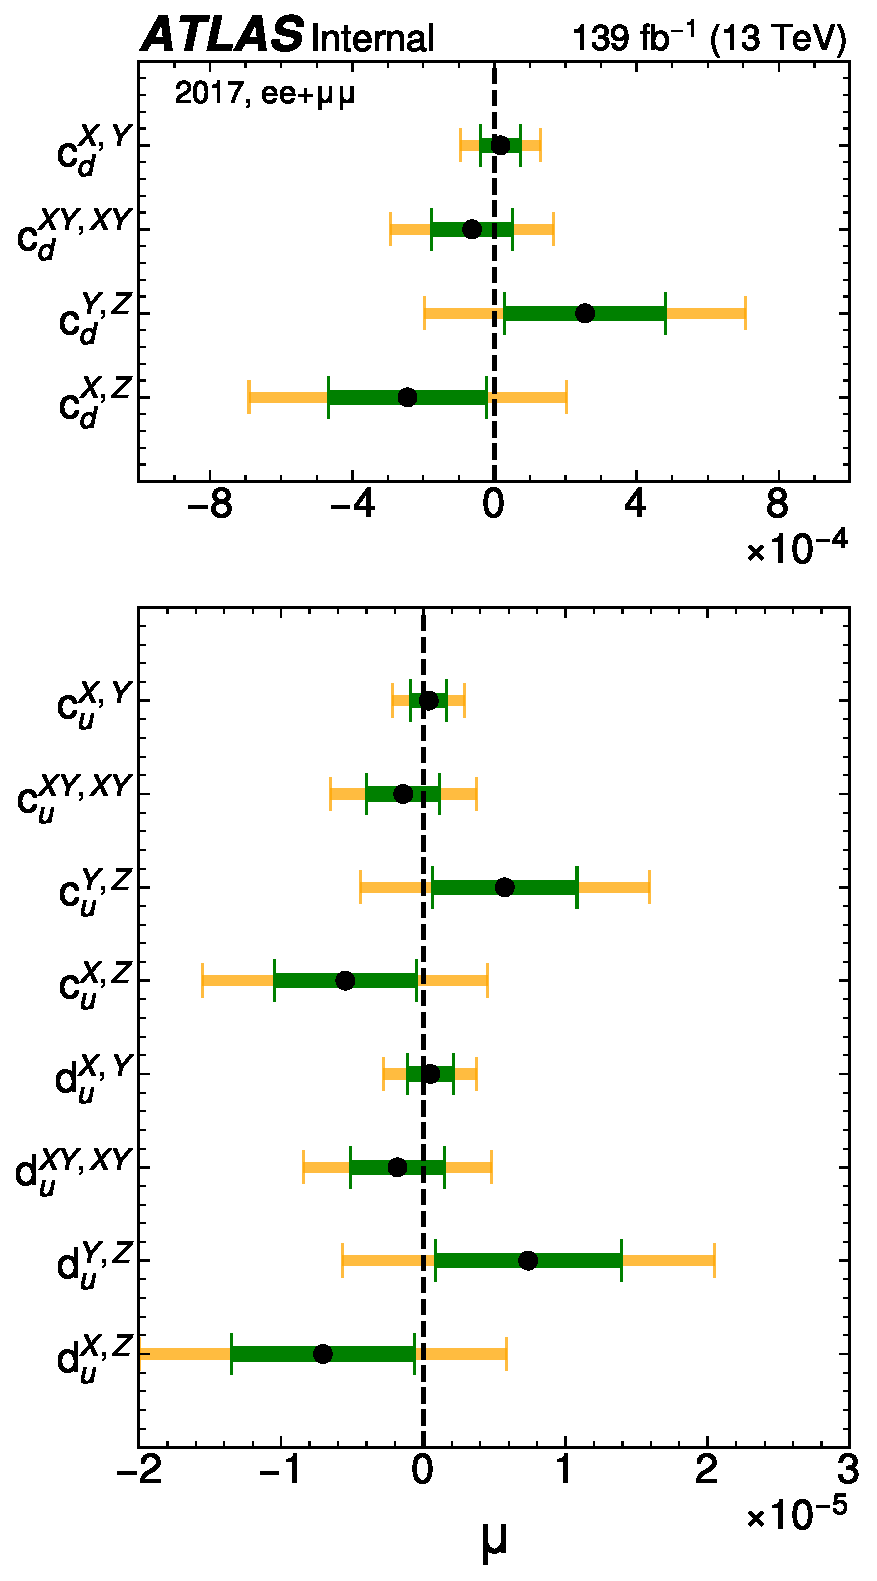
\includegraphics[width=0.30\textwidth]{figs/partially_unblinded_results/SigFit_summary_AllSamples_data17_ll.pdf}
\caption{The scrambled datasets collected in 2017. Plots show average and one (two) standard deviation of 1000 fit results. The black dots are the average values of 1000 fit results, and the green (yellow) band is the corresponding one (two) sigma band. The $ee$ channel is in the left, the $\mu\mu$ channel is in the middle, and the $ee+\mu\mu$ is in the right.}
\label{fig:real_data_scrambled_summary_data17}
\end{figure}

\begin{figure}[ht]
\centering
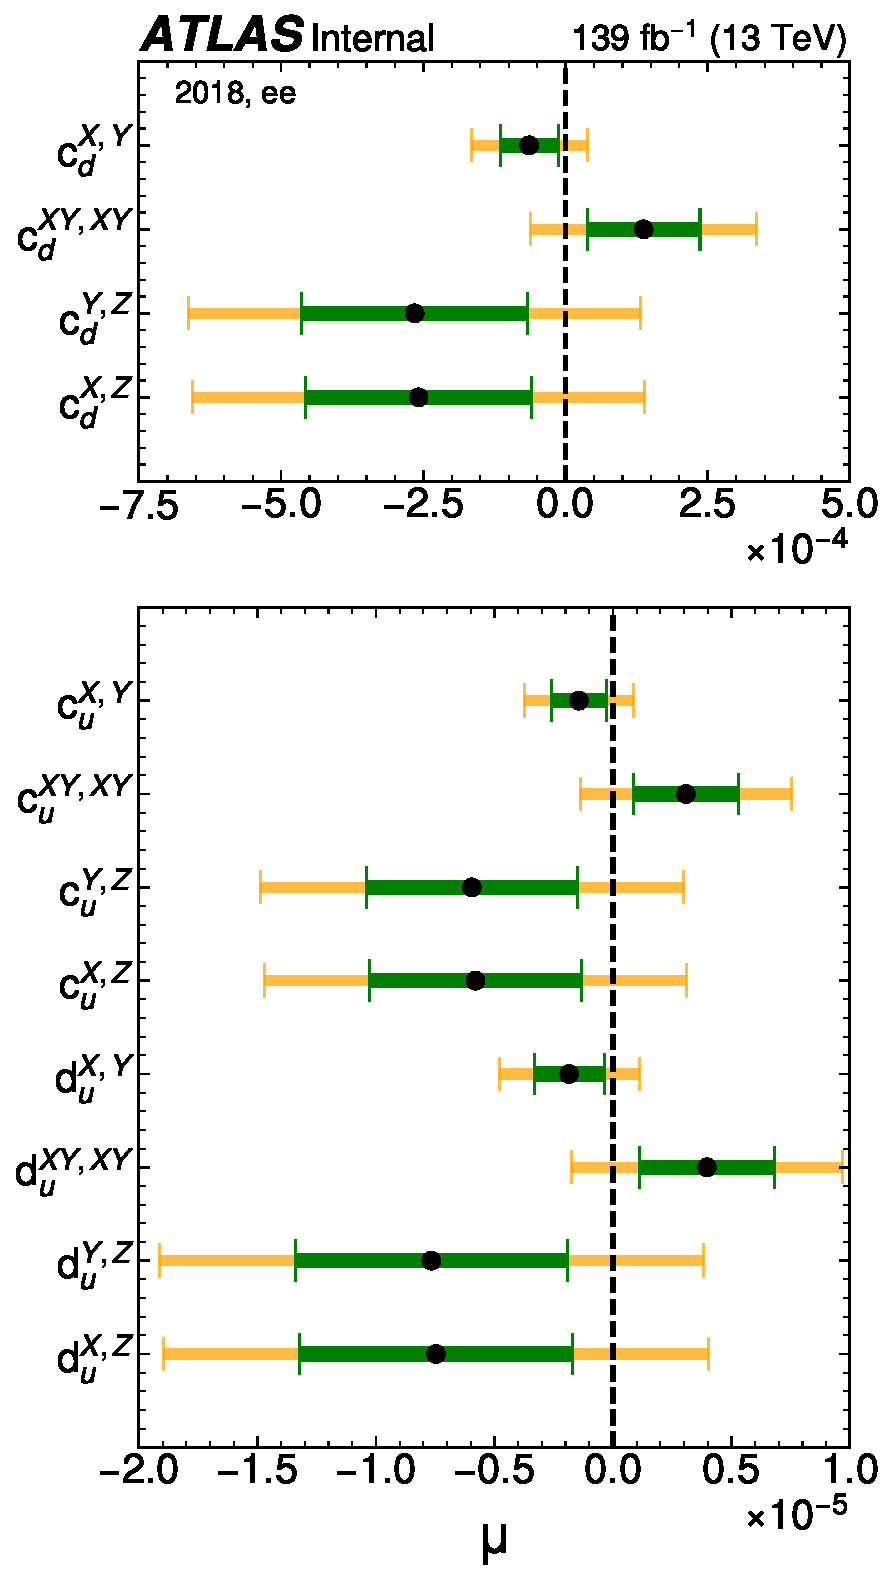
\includegraphics[width=0.30\textwidth]{figs/partially_unblinded_results/SigFit_summary_AllSamples_data18_ee.pdf}
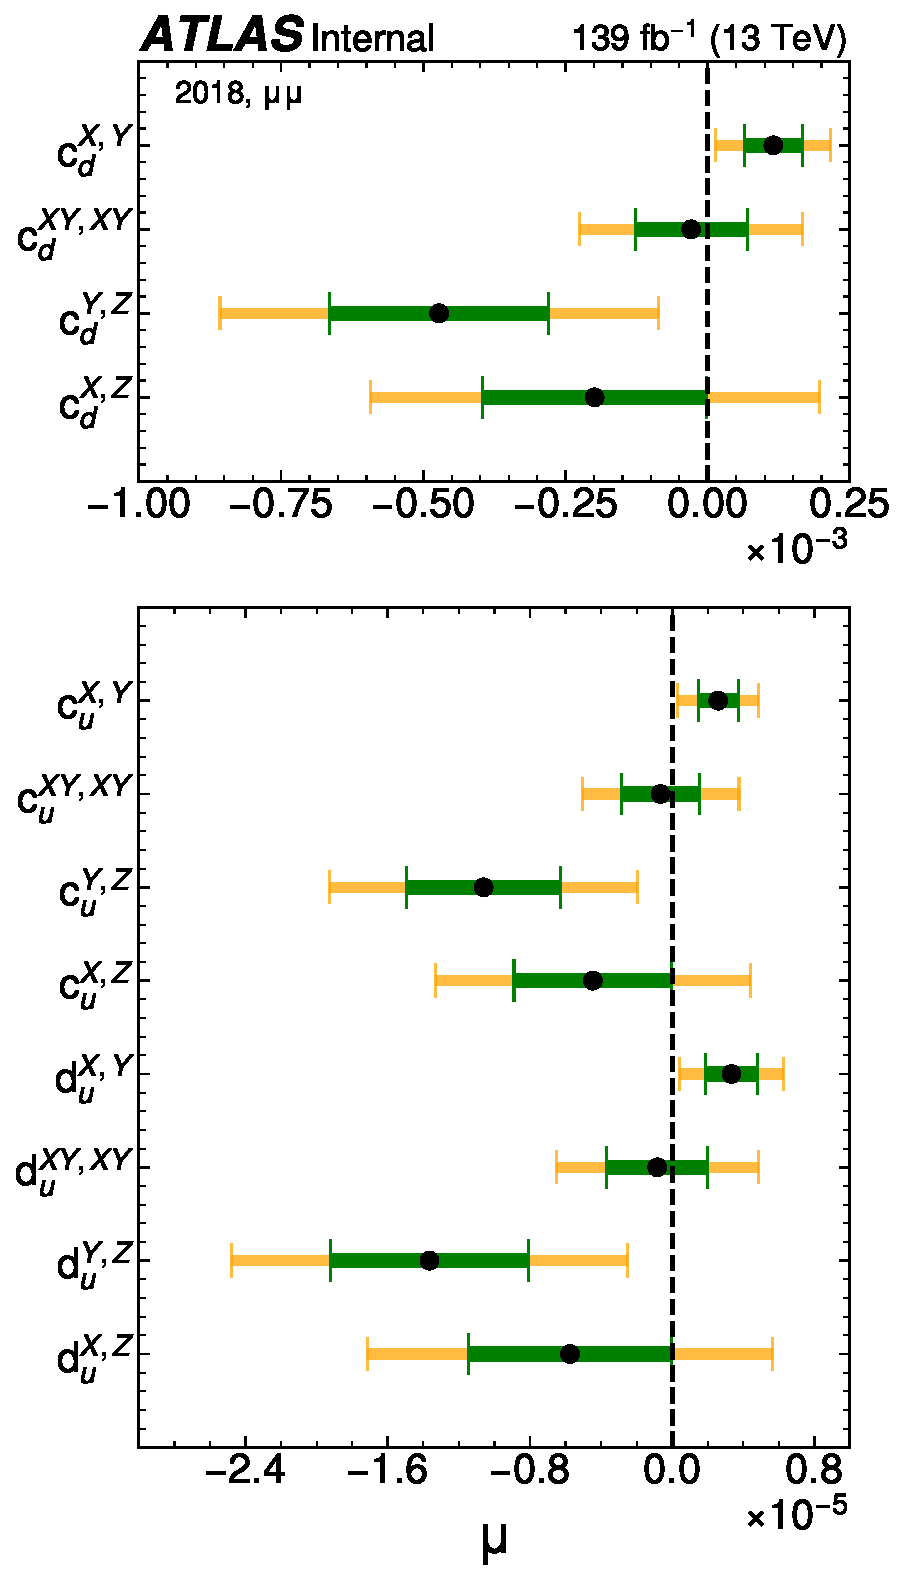
\includegraphics[width=0.30\textwidth]{figs/partially_unblinded_results/SigFit_summary_AllSamples_data18_uu.pdf}
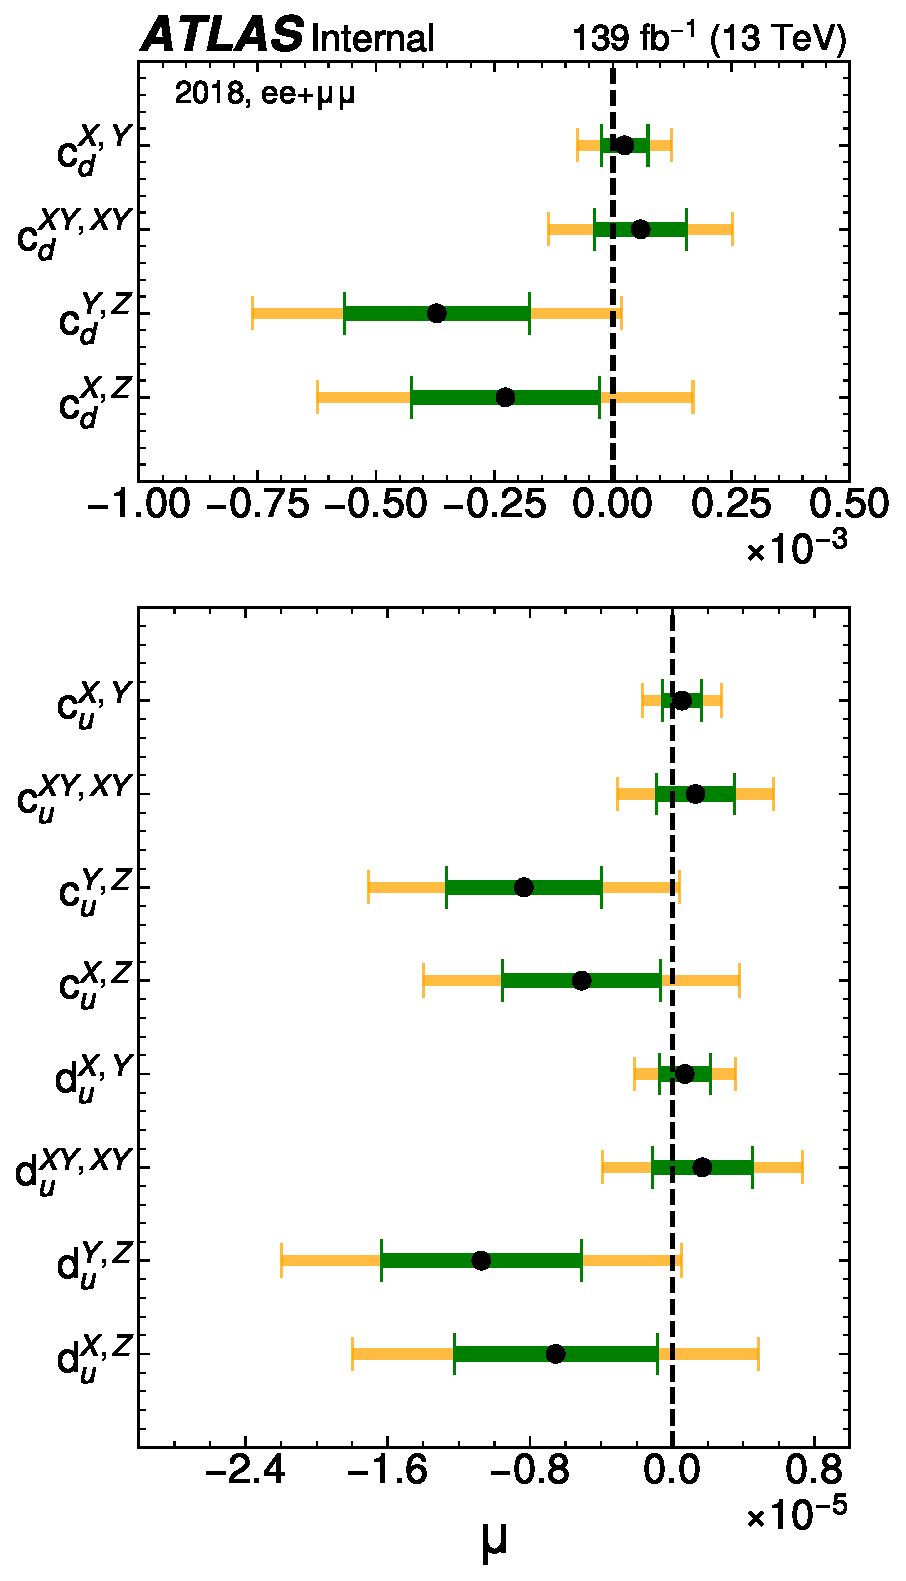
\includegraphics[width=0.30\textwidth]{figs/partially_unblinded_results/SigFit_summary_AllSamples_data18_ll.pdf}
\caption{The scrambled datasets collected in 2018. Plots show average and one (two) standard deviation of 1000 fit results. The black dots are the average values of 1000 fit results, and the green (yellow) band is the corresponding one (two) sigma band. The $ee$ channel is in the left, the $\mu\mu$ channel is in the middle, and the $ee+\mu\mu$ is in the right.}
\label{fig:real_data_scrambled_summary_data18}
\end{figure}


\begin{figure}[ht]
\centering
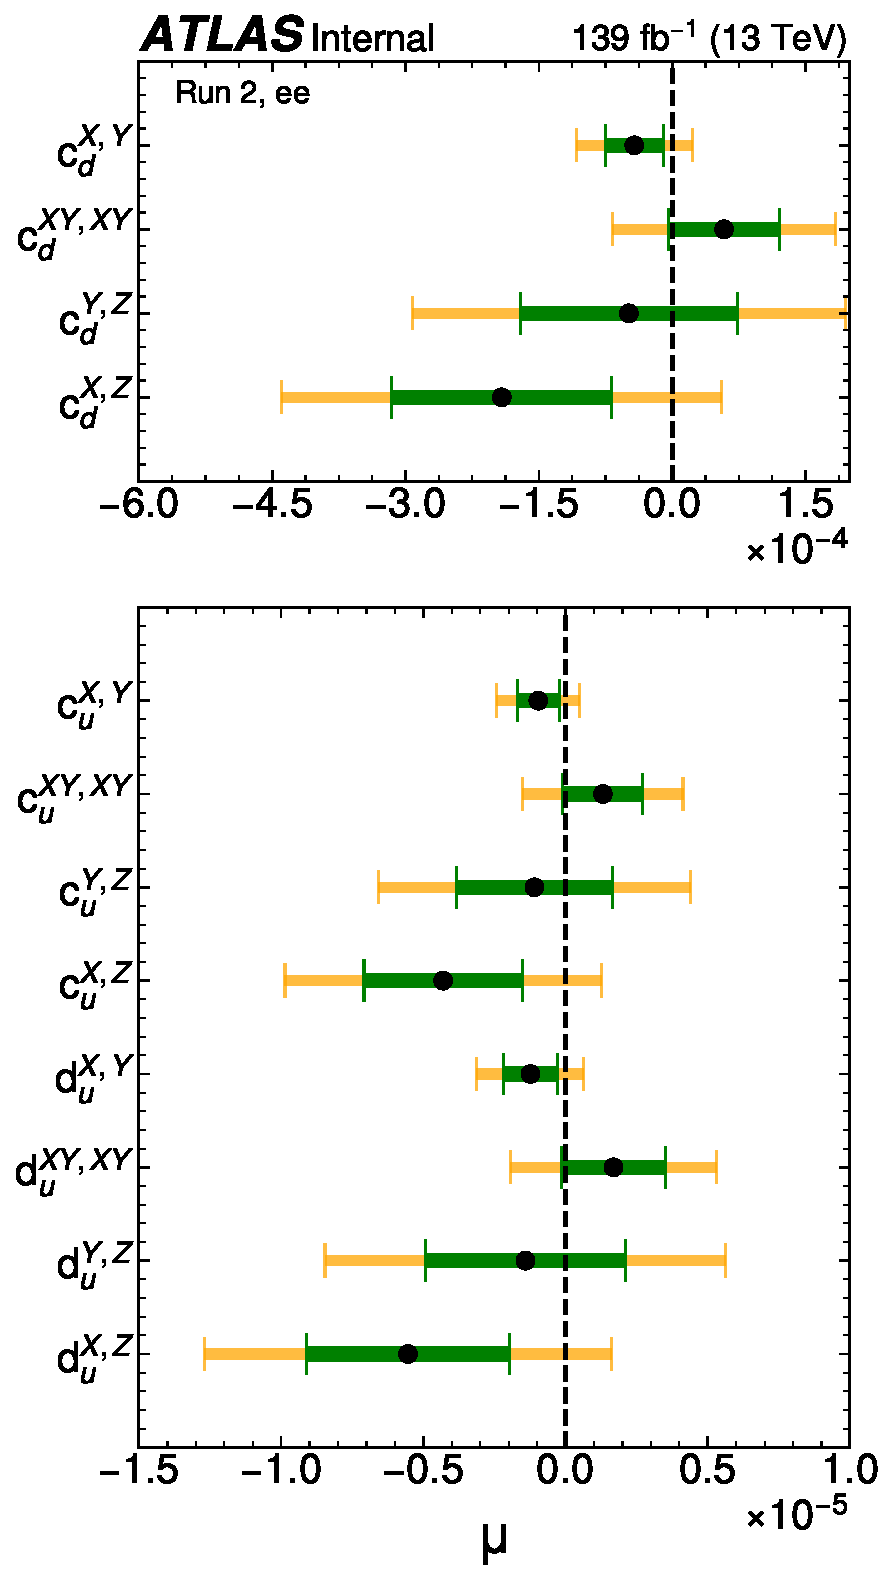
\includegraphics[width=0.30\textwidth]{figs/partially_unblinded_results/SigFit_summary_AllSamples_full_ee.pdf}
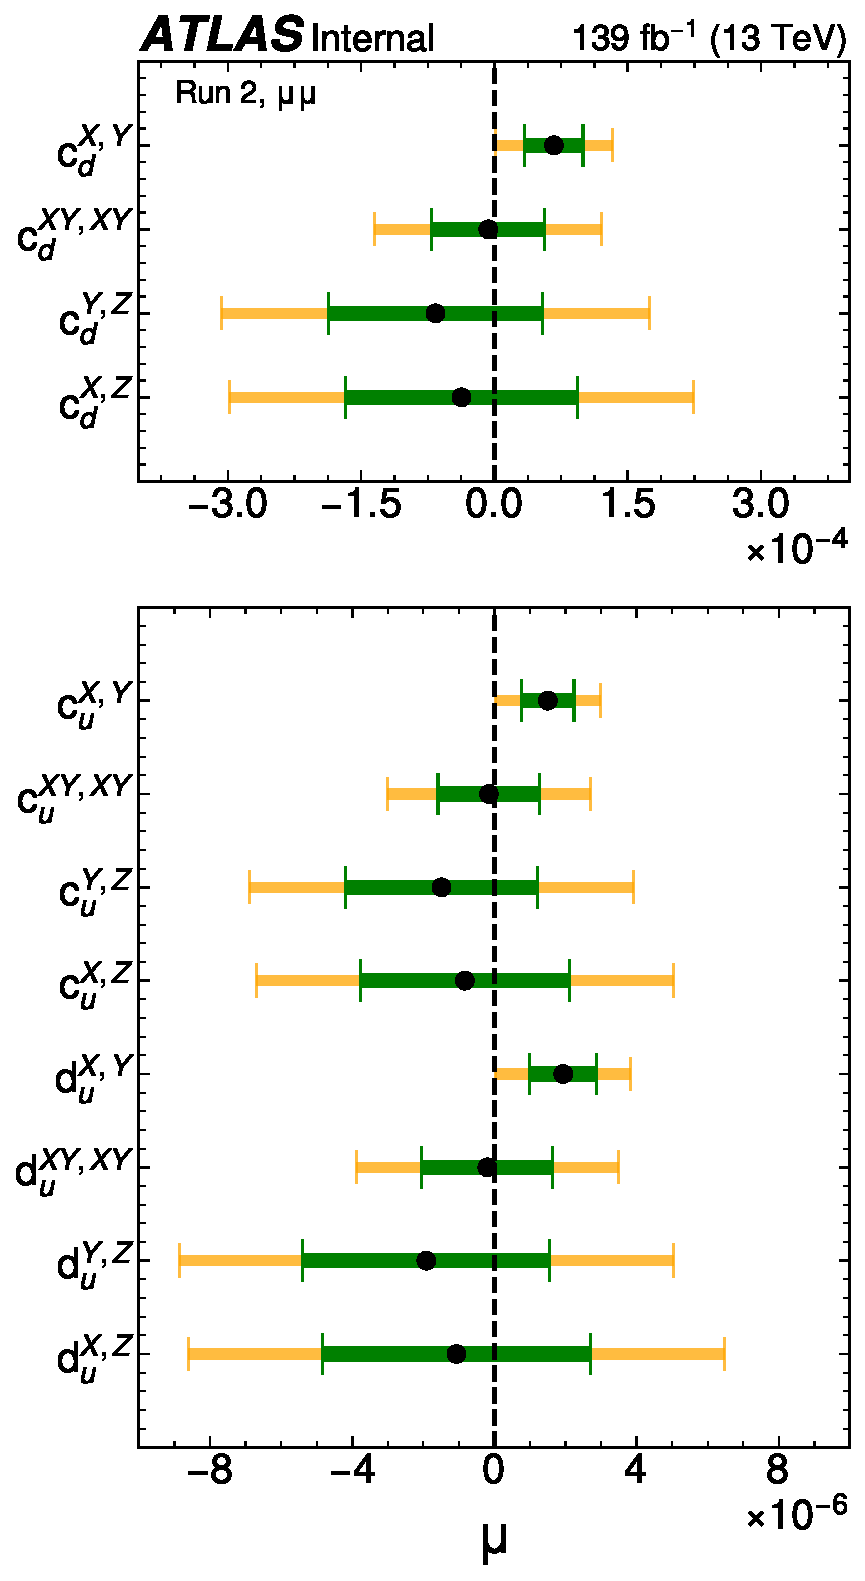
\includegraphics[width=0.30\textwidth]{figs/partially_unblinded_results/SigFit_summary_AllSamples_full_uu.pdf}
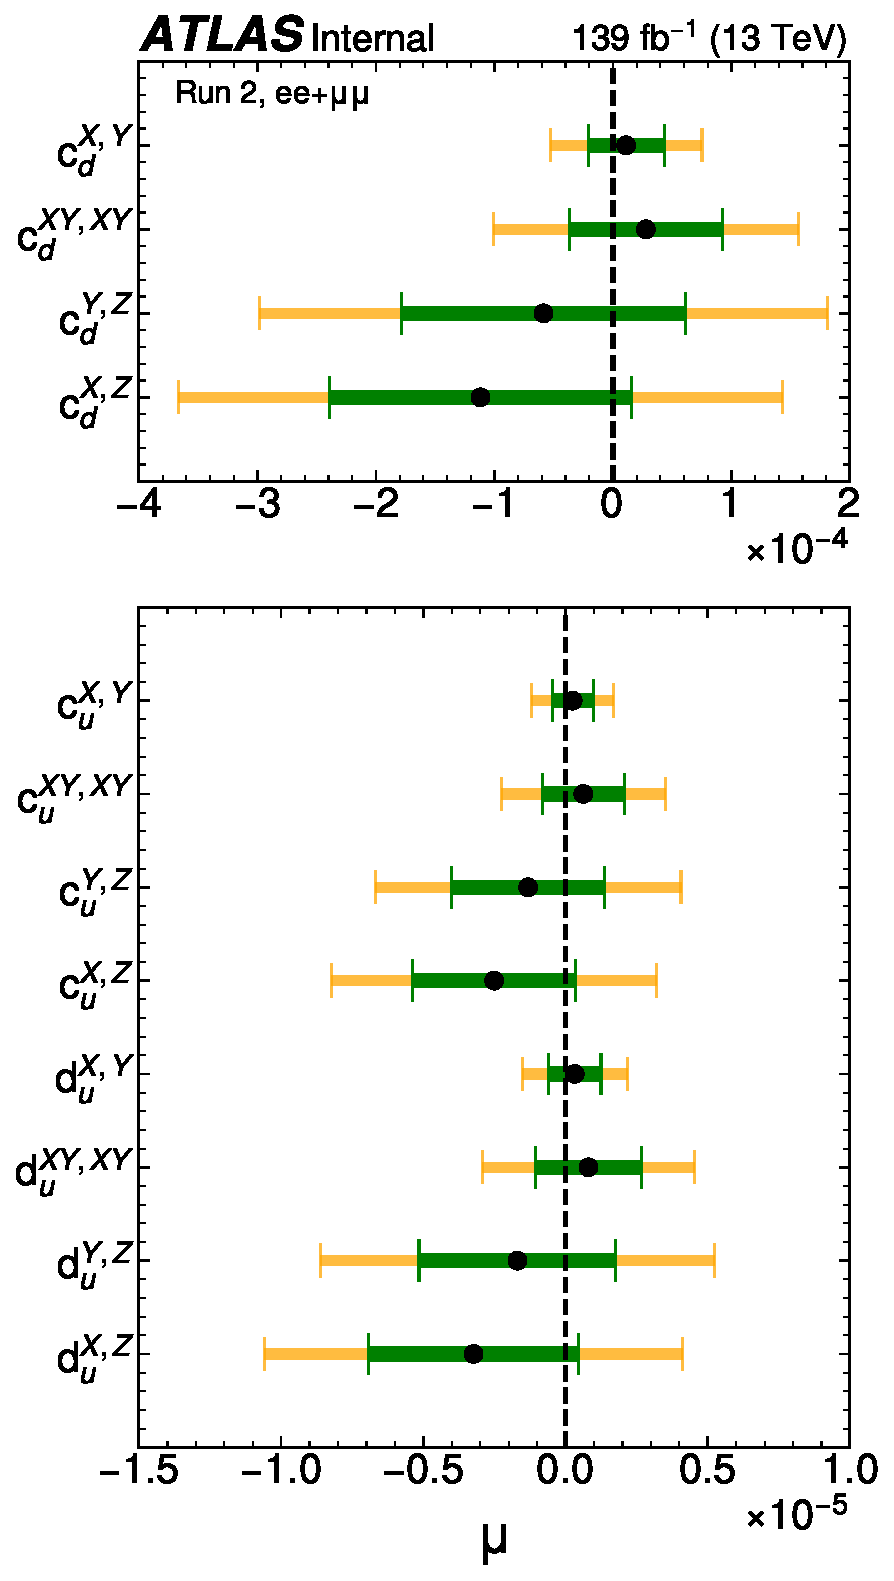
\includegraphics[width=0.30\textwidth]{figs/partially_unblinded_results/SigFit_summary_AllSamples_full_ll.pdf}
\caption{The scrambled datasets in full Run 2 (sum of all years). Plots show average and one (two) standard deviation of 1000 fit results. The black dots are the average values of 1000 fit results, and the green (yellow) band is the corresponding one (two) sigma band. The $ee$ channel is in the left, the $\mu\mu$ channel is in the middle, and the $ee+\mu\mu$ is in the right.}
\label{fig:real_data_scrambled_summary_full}
\end{figure}



\begin{figure}[ht]
\centering
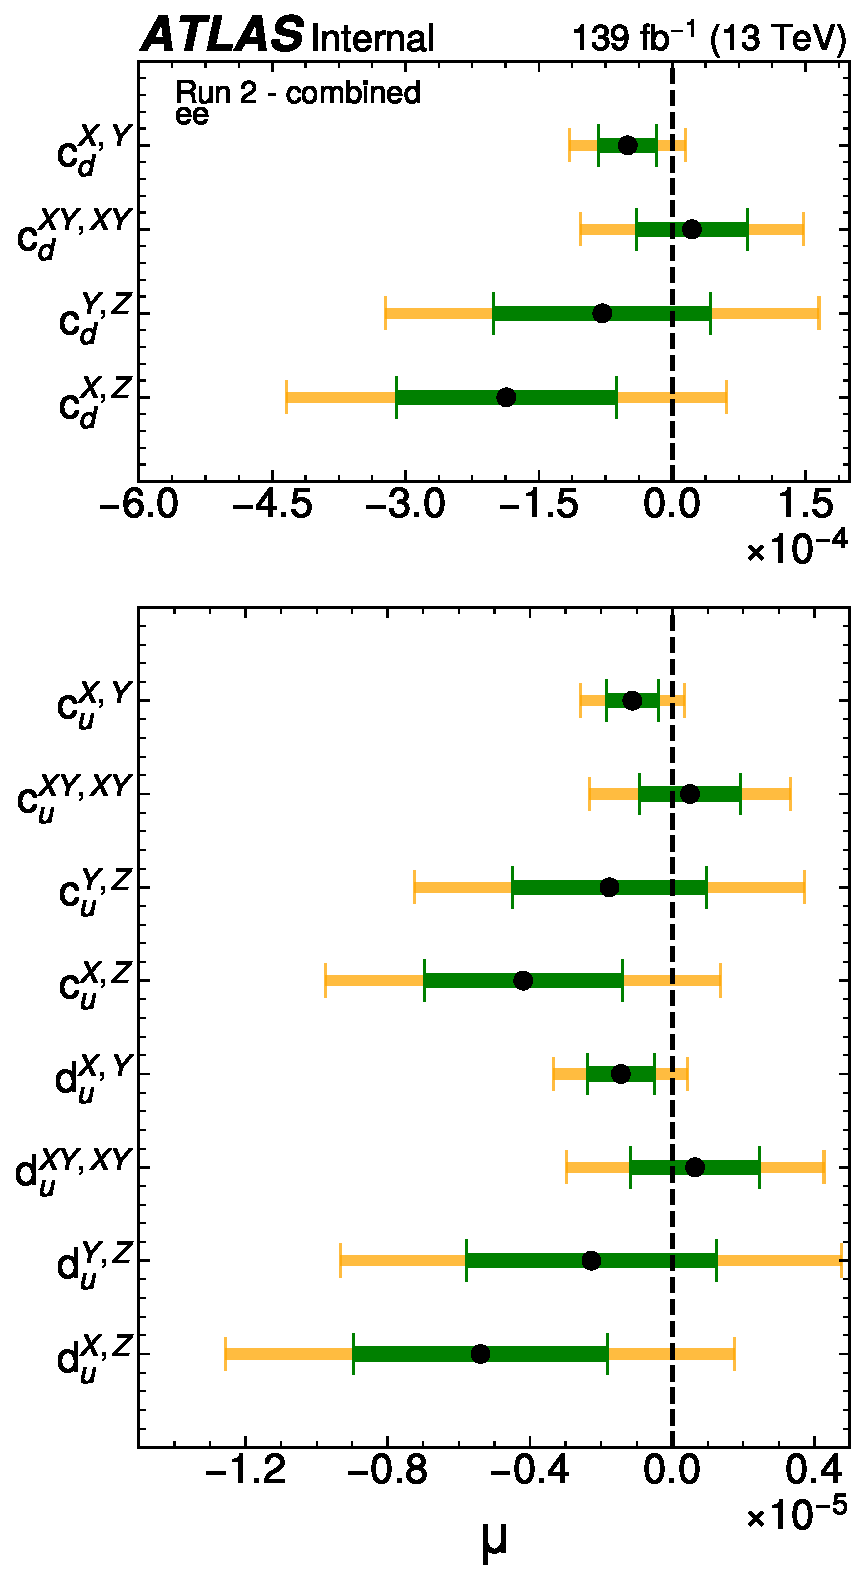
\includegraphics[width=0.30\textwidth]{figs/partially_unblinded_results/SigFit_summary_AllSamples_Combined_ee}
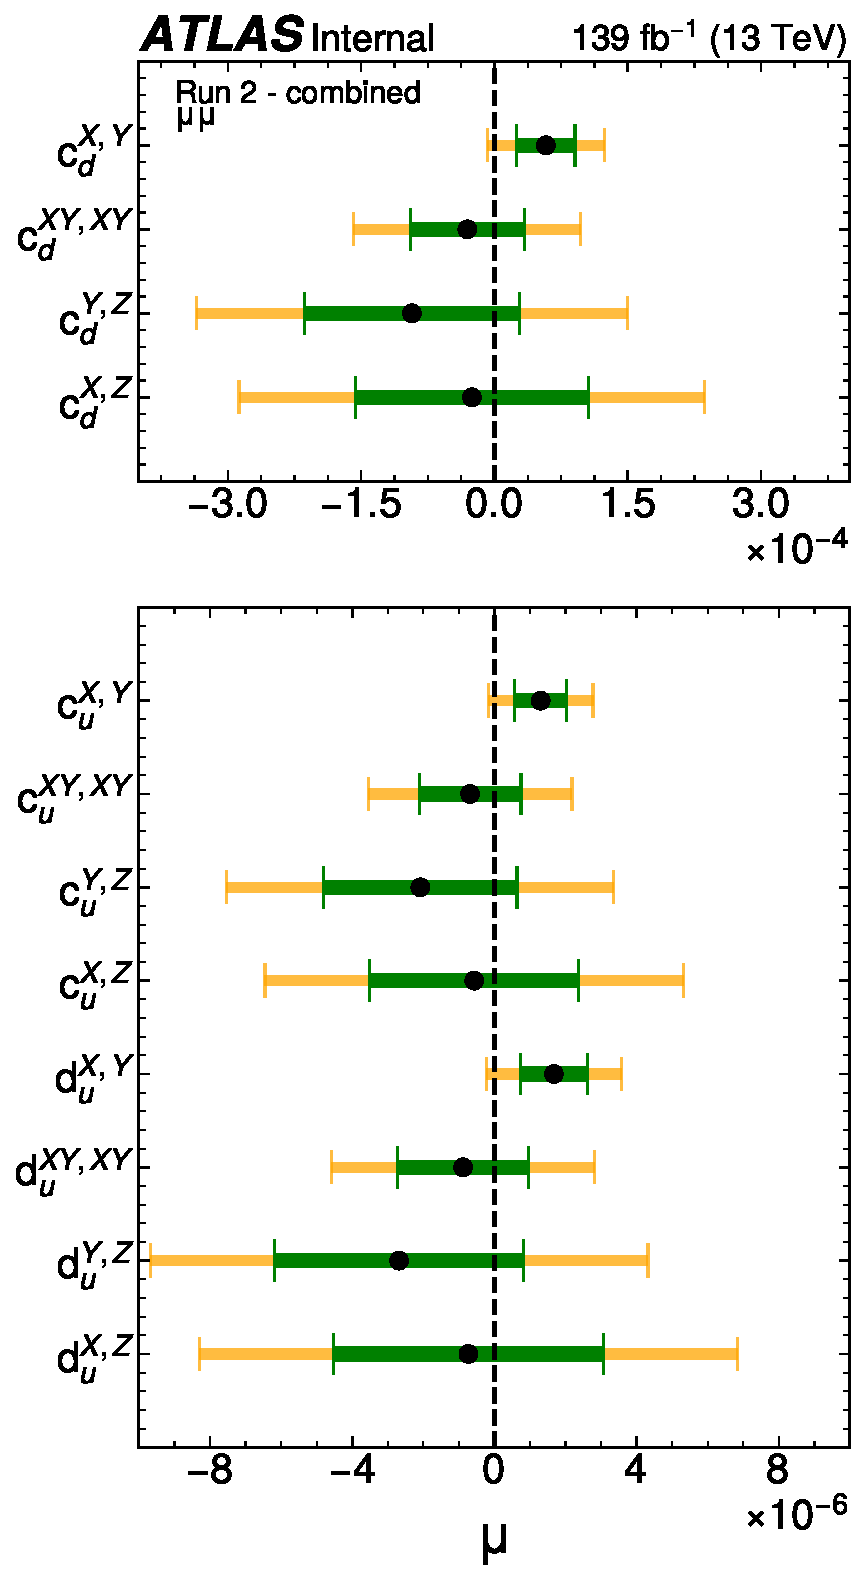
\includegraphics[width=0.30\textwidth]{figs/partially_unblinded_results/SigFit_summary_AllSamples_Combined_uu}
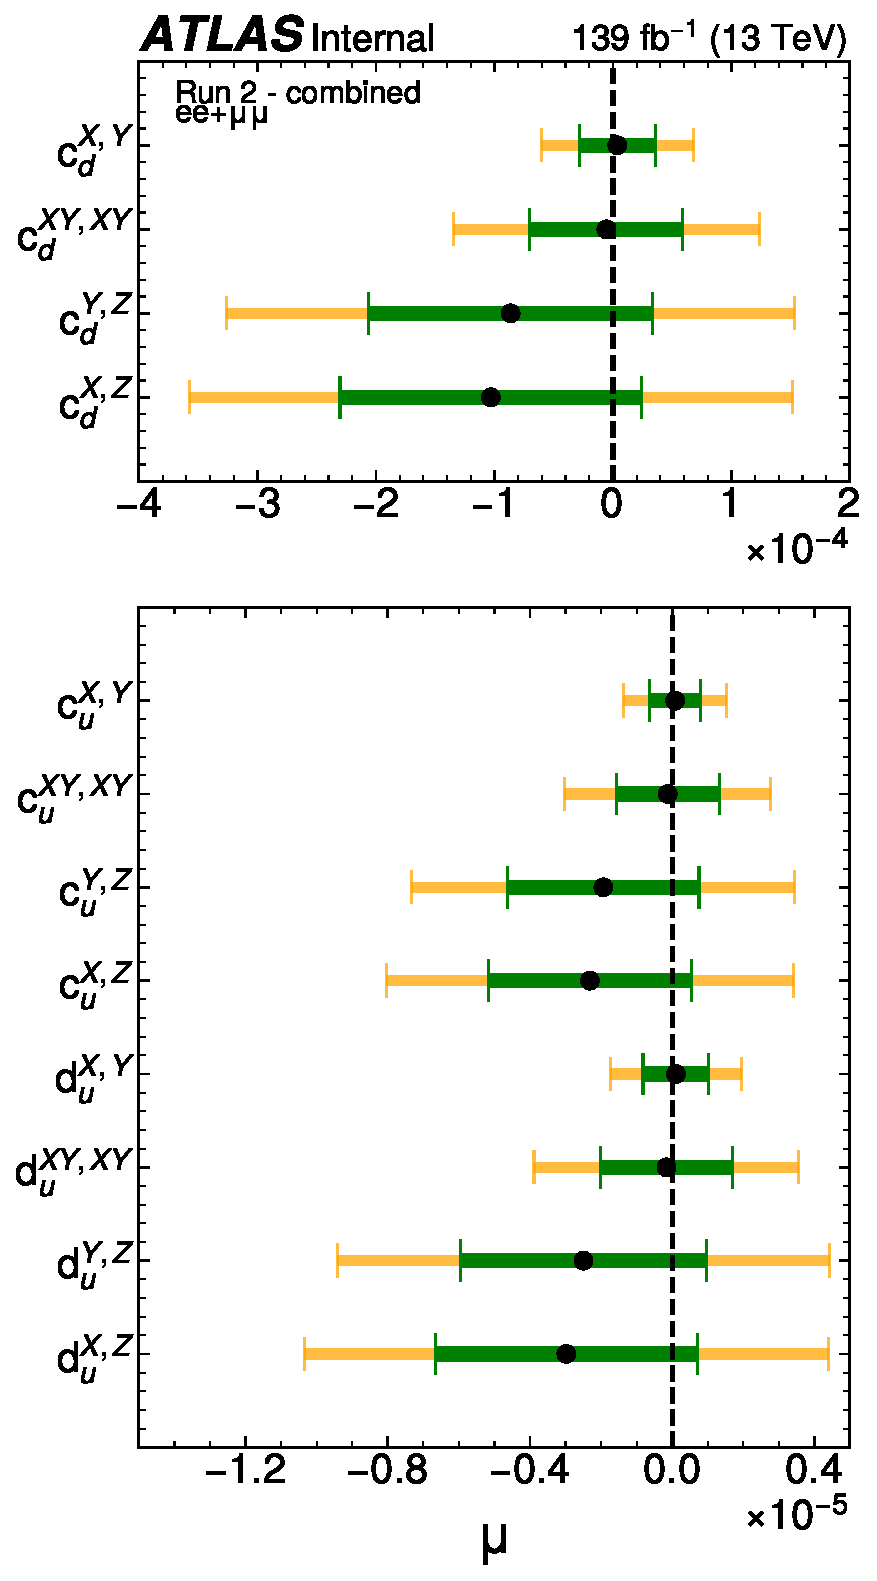
\includegraphics[width=0.30\textwidth]{figs/partially_unblinded_results/SigFit_summary_AllSamples_Combined_ll}
\caption{Run2-combined scrambled datasets. Plots show average and one (two) standard deviation of 1000 fit results. The black dots are the average values of 1000 fit results, and the green (yellow) band is the corresponding one (two) sigma band. The $ee$ channel is in the left, the $\mu\mu$ channel is in the middle, and the $ee+\mu\mu$ is in the right.}
\label{fig:real_data_scrambled_summary_combined}
\end{figure}



\begin{table}[htbp]
\begin{center}
\Rotatebox{90}{%
%%\resizebox{\textwidth}{!}{
\begin{tabular}{|l|c| c| c| c |c|}
\hline
& 2015+2016 & 2017 & 2018 & full Run2 & Run2-Comb. Fit \\
\hline
$d_{\it u}^{\it X,Z}$  & 8.82e-06 $\pm$ 7.44e-06 & -1.42e-05 $\pm$ 6.43e-06 & -7.47e-06 $\pm$ 5.74e-06 & -5.54e-06 $\pm$ 3.58e-06 & -5.39e-06 $\pm$ 3.58e-06 \\
\hline
$d_{\it u}^{\it Y,Z}$  & 1.77e-06 $\pm$ 6.61e-06 & 2.31e-06 $\pm$ 6.61e-06 & -7.67e-06 $\pm$ 5.74e-06 & -1.41e-06 $\pm$ 3.52e-06 & -2.27e-06 $\pm$ 3.52e-06 \\
\hline
$d_{\it u}^{\it XY,XY}$  & -6.12e-06 $\pm$ 3.55e-06 & 2.41e-06 $\pm$ 3.39e-06 & 3.97e-06 $\pm$ 2.87e-06 & 1.69e-06 $\pm$ 1.81e-06 & 6.42e-07 $\pm$ 1.81e-06 \\
\hline
$d_{\it u}^{\it X,Y}$  & -1.93e-06 $\pm$ 1.88e-06 & -6.03e-07 $\pm$ 1.65e-06 & -1.85e-06 $\pm$ 1.48e-06 & -1.24e-06 $\pm$ 9.41e-07 & -1.45e-06 $\pm$ 9.41e-07 \\
\hline
$c_{\it u}^{\it X,Z}$  & 6.85e-06 $\pm$ 5.78e-06 & -1.10e-05 $\pm$ 5.00e-06 & -5.80e-06 $\pm$ 4.46e-06 & -4.31e-06 $\pm$ 2.78e-06 & -4.19e-06 $\pm$ 2.78e-06 \\
\hline
$c_{\it u}^{\it Y,Z}$  & 1.38e-06 $\pm$ 5.13e-06 & 1.79e-06 $\pm$ 5.13e-06 & -5.96e-06 $\pm$ 4.46e-06 & -1.10e-06 $\pm$ 2.74e-06 & -1.77e-06 $\pm$ 2.74e-06 \\
\hline
$c_{\it u}^{\it XY,XY}$  & -4.76e-06 $\pm$ 2.76e-06 & 1.87e-06 $\pm$ 2.64e-06 & 3.08e-06 $\pm$ 2.23e-06 & 1.31e-06 $\pm$ 1.41e-06 & 4.99e-07 $\pm$ 1.41e-06 \\
\hline
$c_{\it u}^{\it X,Y}$  & -1.50e-06 $\pm$ 1.46e-06 & -4.69e-07 $\pm$ 1.29e-06 & -1.44e-06 $\pm$ 1.15e-06 & -9.60e-07 $\pm$ 7.31e-07 & -1.12e-06 $\pm$ 7.31e-07 \\
\hline
$c_{\it d}^{\it X,Z}$  & 3.05e-04 $\pm$ 2.57e-04 & -4.91e-04 $\pm$ 2.23e-04 & -2.58e-04 $\pm$ 1.99e-04 & -1.92e-04 $\pm$ 1.24e-04 & -1.87e-04 $\pm$ 1.24e-04 \\
\hline
$c_{\it d}^{\it Y,Z}$  & 6.13e-05 $\pm$ 2.29e-04 & 7.98e-05 $\pm$ 2.29e-04 & -2.65e-04 $\pm$ 1.99e-04 & -4.88e-05 $\pm$ 1.22e-04 & -7.87e-05 $\pm$ 1.22e-04 \\
\hline
$c_{\it d}^{\it XY,XY}$  & -2.12e-04 $\pm$ 1.23e-04 & 8.33e-05 $\pm$ 1.17e-04 & 1.37e-04 $\pm$ 9.91e-05 & 5.84e-05 $\pm$ 6.28e-05 & 2.22e-05 $\pm$ 6.28e-05 \\
\hline
$c_{\it d}^{\it X,Y}$  & -6.67e-05 $\pm$ 6.50e-05 & -2.09e-05 $\pm$ 5.72e-05 & -6.40e-05 $\pm$ 5.11e-05 & -4.27e-05 $\pm$ 3.25e-05 & -5.00e-05 $\pm$ 3.25e-05 \\
\hline
\hline
\end{tabular}
}%
\end{center}
\caption{
Partially unblinded results in $ee$ channel. The table shows the average and one standard deviation of 1000 fit results.
\label{table.results}}
\end{table}
%




\newpage


\begin{table}[htbp]
\begin{center}
\Rotatebox{90}{%
%%\resizebox{\textwidth}{!}{
\begin{tabular}{|l|c| c| c| c |c|}
\hline
& 2015+2016 & 2017 & 2018 & full Run2 & Run2-Comb. Fit \\
\hline
$d_{\it u}^{\it X,Z}$  & 6.06e-06 $\pm$ 7.42e-06 & -2.01e-07 $\pm$ 6.46e-06 & -5.75e-06 $\pm$ 5.71e-06 & -1.07e-06 $\pm$ 3.77e-06 & -7.33e-07 $\pm$ 3.79e-06 \\
\hline
$d_{\it u}^{\it Y,Z}$  & -2.57e-06 $\pm$ 7.12e-06 & 1.22e-05 $\pm$ 6.50e-06 & -1.37e-05 $\pm$ 5.57e-06 & -1.92e-06 $\pm$ 3.48e-06 & -2.68e-06 $\pm$ 3.50e-06 \\
\hline
$d_{\it u}^{\it XY,XY}$  & 4.92e-06 $\pm$ 3.56e-06 & -6.05e-06 $\pm$ 3.48e-06 & -8.44e-07 $\pm$ 2.84e-06 & -2.02e-07 $\pm$ 1.84e-06 & -8.82e-07 $\pm$ 1.84e-06 \\
\hline
$d_{\it u}^{\it X,Y}$  & -7.66e-07 $\pm$ 1.86e-06 & 1.71e-06 $\pm$ 1.67e-06 & 3.33e-06 $\pm$ 1.46e-06 & 1.93e-06 $\pm$ 9.46e-07 & 1.67e-06 $\pm$ 9.48e-07 \\
\hline
$c_{\it u}^{\it X,Z}$  & 4.71e-06 $\pm$ 5.76e-06 & -1.56e-07 $\pm$ 5.02e-06 & -4.47e-06 $\pm$ 4.43e-06 & -8.31e-07 $\pm$ 2.93e-06 & -5.69e-07 $\pm$ 2.94e-06 \\
\hline
$c_{\it u}^{\it Y,Z}$  & -1.99e-06 $\pm$ 5.53e-06 & 9.46e-06 $\pm$ 5.05e-06 & -1.06e-05 $\pm$ 4.33e-06 & -1.49e-06 $\pm$ 2.70e-06 & -2.09e-06 $\pm$ 2.72e-06 \\
\hline
$c_{\it u}^{\it XY,XY}$  & 3.82e-06 $\pm$ 2.77e-06 & -4.70e-06 $\pm$ 2.70e-06 & -6.55e-07 $\pm$ 2.21e-06 & -1.57e-07 $\pm$ 1.43e-06 & -6.85e-07 $\pm$ 1.43e-06 \\
\hline
$c_{\it u}^{\it X,Y}$  & -5.95e-07 $\pm$ 1.44e-06 & 1.33e-06 $\pm$ 1.30e-06 & 2.59e-06 $\pm$ 1.13e-06 & 1.50e-06 $\pm$ 7.35e-07 & 1.30e-06 $\pm$ 7.37e-07 \\
\hline
$c_{\it d}^{\it X,Z}$  & 2.10e-04 $\pm$ 2.57e-04 & -6.94e-06 $\pm$ 2.24e-04 & -1.99e-04 $\pm$ 1.97e-04 & -3.70e-05 $\pm$ 1.31e-04 & -2.54e-05 $\pm$ 1.31e-04 \\
\hline
$c_{\it d}^{\it Y,Z}$  & -8.88e-05 $\pm$ 2.46e-04 & 4.21e-04 $\pm$ 2.25e-04 & -4.72e-04 $\pm$ 1.93e-04 & -6.63e-05 $\pm$ 1.20e-04 & -9.29e-05 $\pm$ 1.21e-04 \\
\hline
$c_{\it d}^{\it XY,XY}$  & 1.70e-04 $\pm$ 1.23e-04 & -2.09e-04 $\pm$ 1.20e-04 & -2.92e-05 $\pm$ 9.83e-05 & -6.97e-06 $\pm$ 6.38e-05 & -3.05e-05 $\pm$ 6.38e-05 \\
\hline
$c_{\it d}^{\it X,Y}$  & -2.65e-05 $\pm$ 6.42e-05 & 5.92e-05 $\pm$ 5.78e-05 & 1.15e-04 $\pm$ 5.05e-05 & 6.69e-05 $\pm$ 3.27e-05 & 5.78e-05 $\pm$ 3.28e-05 \\
\hline
\hline
\end{tabular}
}%
\end{center}
\caption{
Partially unblinded results in $\mu\mu$ channel. The table shows the average and one standard deviation of 1000 fit results.
\label{table.results}}
\end{table}
%


\newpage


\begin{table}[htbp]
\begin{center}
\Rotatebox{90}{%
%%\resizebox{\textwidth}{!}{
\begin{tabular}{|l|c| c| c| c |c|}
\hline
 & 2015+2016 & 2017 & 2018 & full Run2 & Run2-Comb. Fit \\
\hline
$d_{\it u}^{\it X,Z}$  & 7.48e-06 $\pm$ 7.22e-06 & -7.07e-06 $\pm$ 6.44e-06 & -6.56e-06 $\pm$ 5.72e-06 & -3.23e-06 $\pm$ 3.68e-06 & -2.98e-06 $\pm$ 3.68e-06 \\
\hline
$d_{\it u}^{\it Y,Z}$  & -5.06e-07 $\pm$ 7.16e-06 & 7.37e-06 $\pm$ 6.54e-06 & -1.07e-05 $\pm$ 5.63e-06 & -1.69e-06 $\pm$ 3.46e-06 & -2.49e-06 $\pm$ 3.46e-06 \\
\hline
$d_{\it u}^{\it XY,XY}$  & -5.76e-07 $\pm$ 3.72e-06 & -1.82e-06 $\pm$ 3.31e-06 & 1.69e-06 $\pm$ 2.81e-06 & 8.03e-07 $\pm$ 1.86e-06 & -1.62e-07 $\pm$ 1.86e-06 \\
\hline
$d_{\it u}^{\it X,Y}$  & -1.35e-06 $\pm$ 1.93e-06 & 4.94e-07 $\pm$ 1.63e-06 & 7.10e-07 $\pm$ 1.43e-06 & 3.21e-07 $\pm$ 9.25e-07 & 1.05e-07 $\pm$ 9.27e-07 \\
\hline
$c_{\it u}^{\it X,Z}$  & 5.81e-06 $\pm$ 5.61e-06 & -5.49e-06 $\pm$ 5.01e-06 & -5.09e-06 $\pm$ 4.44e-06 & -2.51e-06 $\pm$ 2.86e-06 & -2.31e-06 $\pm$ 2.86e-06 \\
\hline
$c_{\it u}^{\it Y,Z}$  & -3.93e-07 $\pm$ 5.57e-06 & 5.73e-06 $\pm$ 5.08e-06 & -8.35e-06 $\pm$ 4.37e-06 & -1.32e-06 $\pm$ 2.69e-06 & -1.94e-06 $\pm$ 2.69e-06 \\
\hline
$c_{\it u}^{\it XY,XY}$  & -4.48e-07 $\pm$ 2.89e-06 & -1.42e-06 $\pm$ 2.57e-06 & 1.31e-06 $\pm$ 2.18e-06 & 6.24e-07 $\pm$ 1.44e-06 & -1.26e-07 $\pm$ 1.45e-06 \\
\hline
$c_{\it u}^{\it X,Y}$  & -1.05e-06 $\pm$ 1.50e-06 & 3.84e-07 $\pm$ 1.27e-06 & 5.51e-07 $\pm$ 1.11e-06 & 2.50e-07 $\pm$ 7.19e-07 & 8.17e-08 $\pm$ 7.20e-07 \\
\hline
$c_{\it d}^{\it X,Z}$  & 2.59e-04 $\pm$ 2.50e-04 & -2.44e-04 $\pm$ 2.23e-04 & -2.27e-04 $\pm$ 1.98e-04 & -1.12e-04 $\pm$ 1.27e-04 & -1.03e-04 $\pm$ 1.27e-04 \\
\hline
$c_{\it d}^{\it Y,Z}$  & -1.75e-05 $\pm$ 2.48e-04 & 2.55e-04 $\pm$ 2.26e-04 & -3.72e-04 $\pm$ 1.95e-04 & -5.86e-05 $\pm$ 1.20e-04 & -8.63e-05 $\pm$ 1.20e-04 \\
\hline
$c_{\it d}^{\it XY,XY}$  & -1.99e-05 $\pm$ 1.29e-04 & -6.30e-05 $\pm$ 1.14e-04 & 5.85e-05 $\pm$ 9.73e-05 & 2.78e-05 $\pm$ 6.43e-05 & -5.59e-06 $\pm$ 6.45e-05 \\
\hline
$c_{\it d}^{\it X,Y}$  & -4.66e-05 $\pm$ 6.66e-05 & 1.71e-05 $\pm$ 5.65e-05 & 2.46e-05 $\pm$ 4.93e-05 & 1.11e-05 $\pm$ 3.20e-05 & 3.64e-06 $\pm$ 3.21e-05 \\
\hline
\hline
\end{tabular}
}%
\end{center}
\caption{
Partially unblinded results in $ee+\mu\mu$ channel. The table shows the average and one standard deviation of 1000 fit results.
\label{table.results}}
\end{table}
%

\subsubsection{Spread VS Stats}



\begin{figure}[ht]
\centering
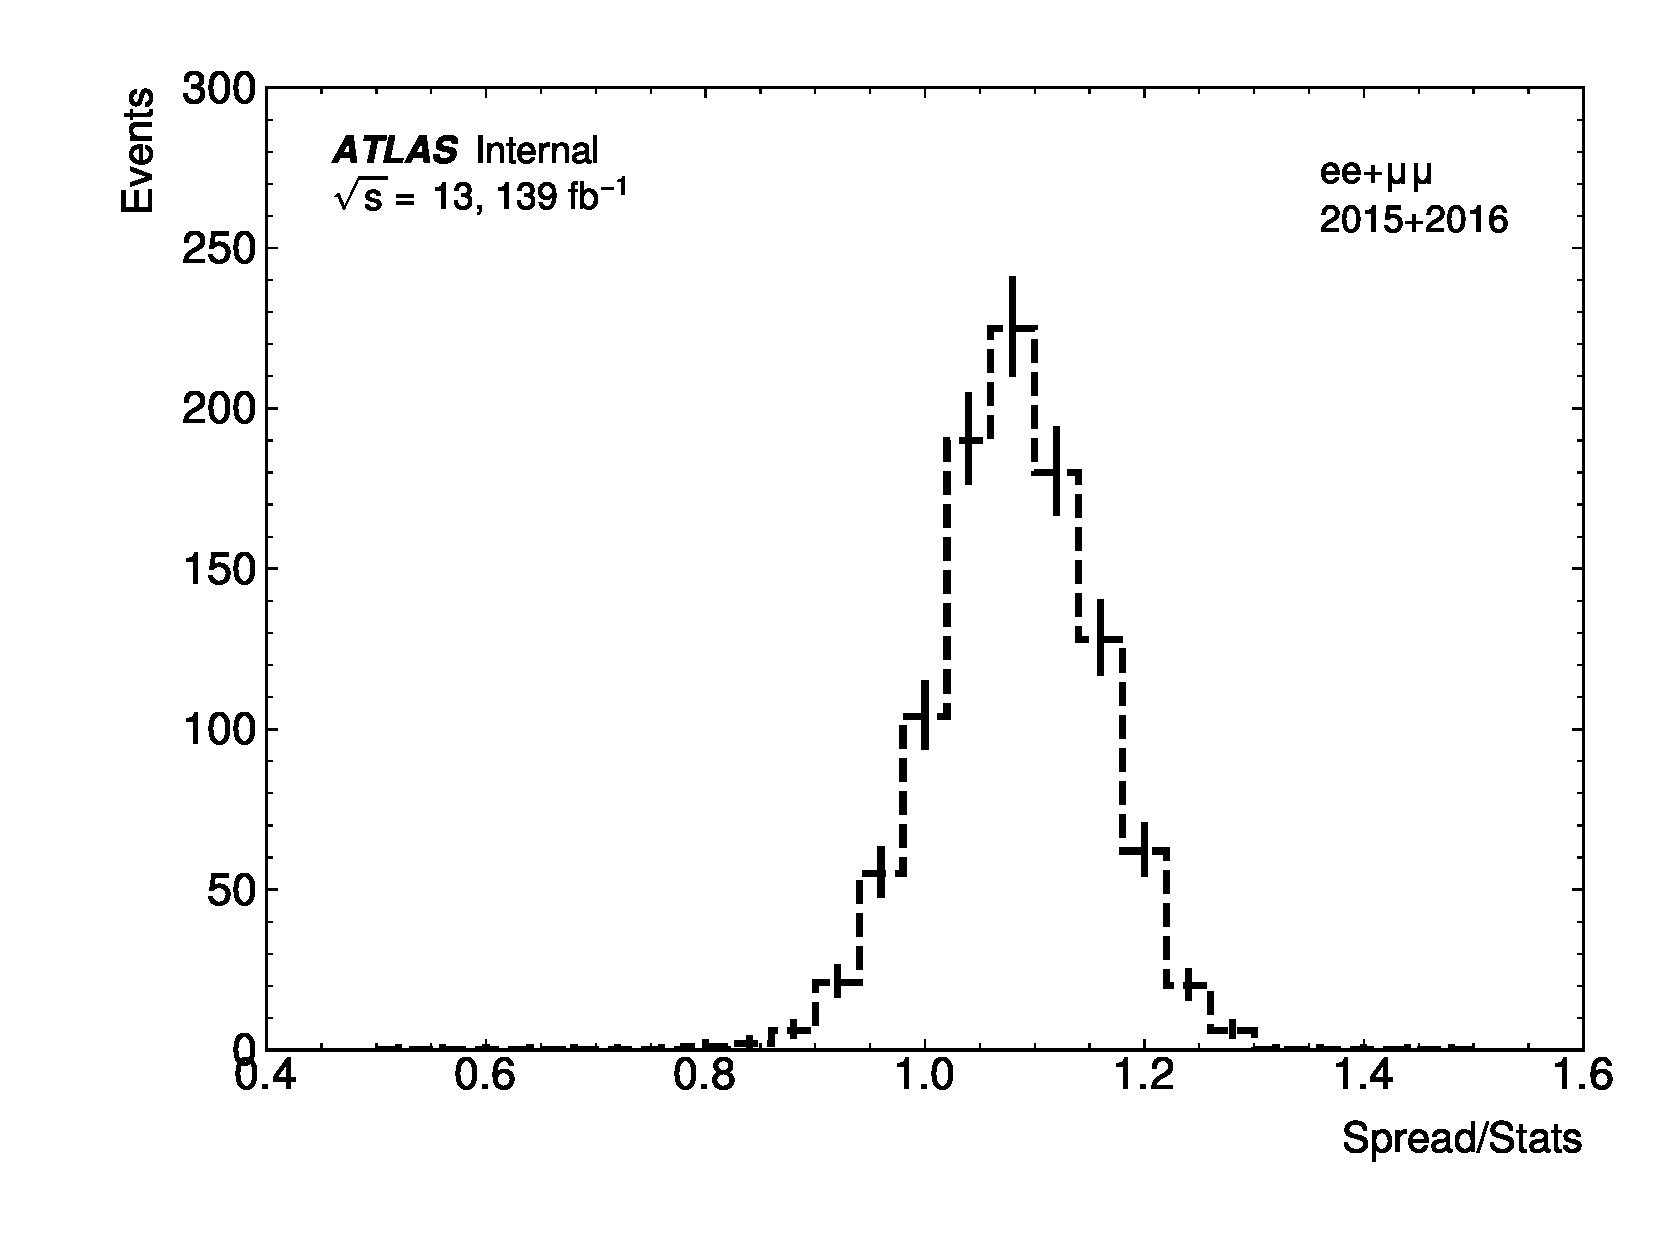
\includegraphics[width=0.45\textwidth]{figs/partially_unblinded_results/spread_stats_scrambled_data15p16_Ratio.pdf}
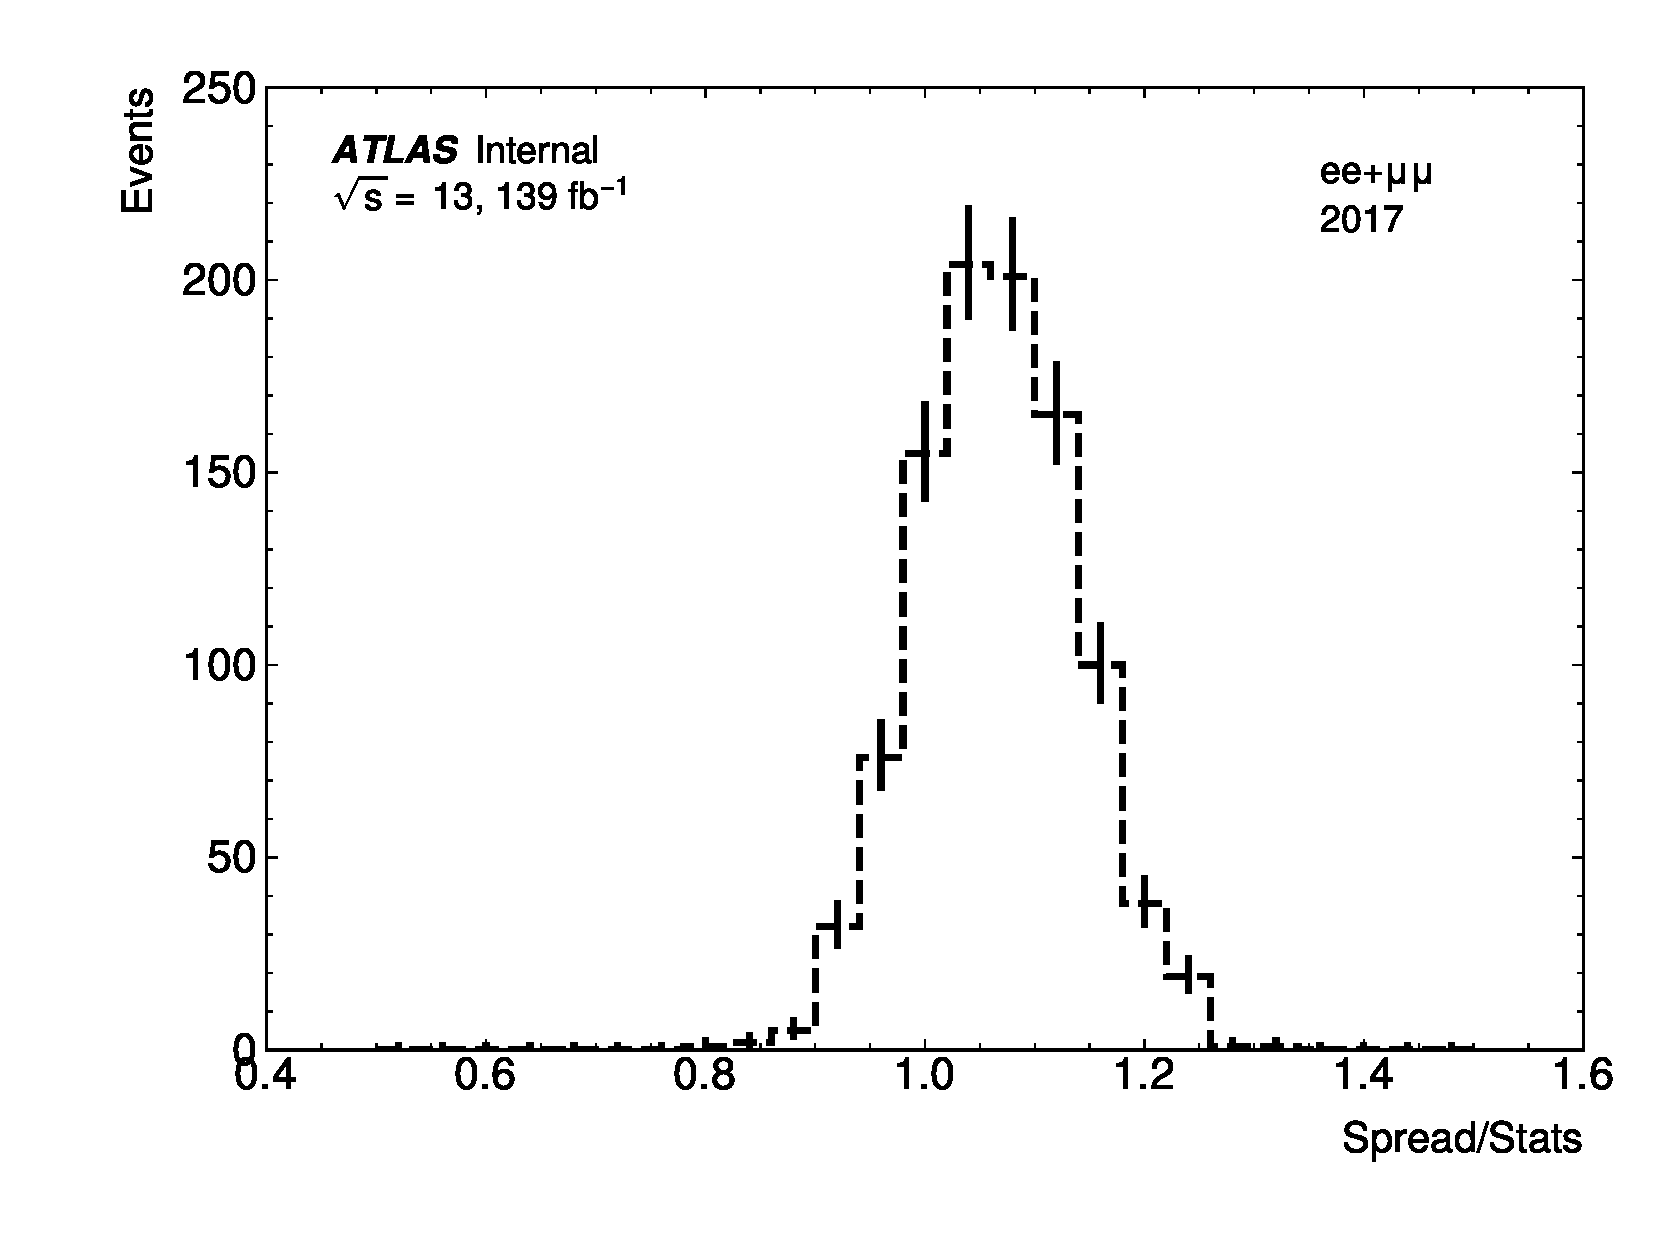
\includegraphics[width=0.45\textwidth]{figs/partially_unblinded_results/spread_stats_scrambled_data17_Ratio.pdf}\\
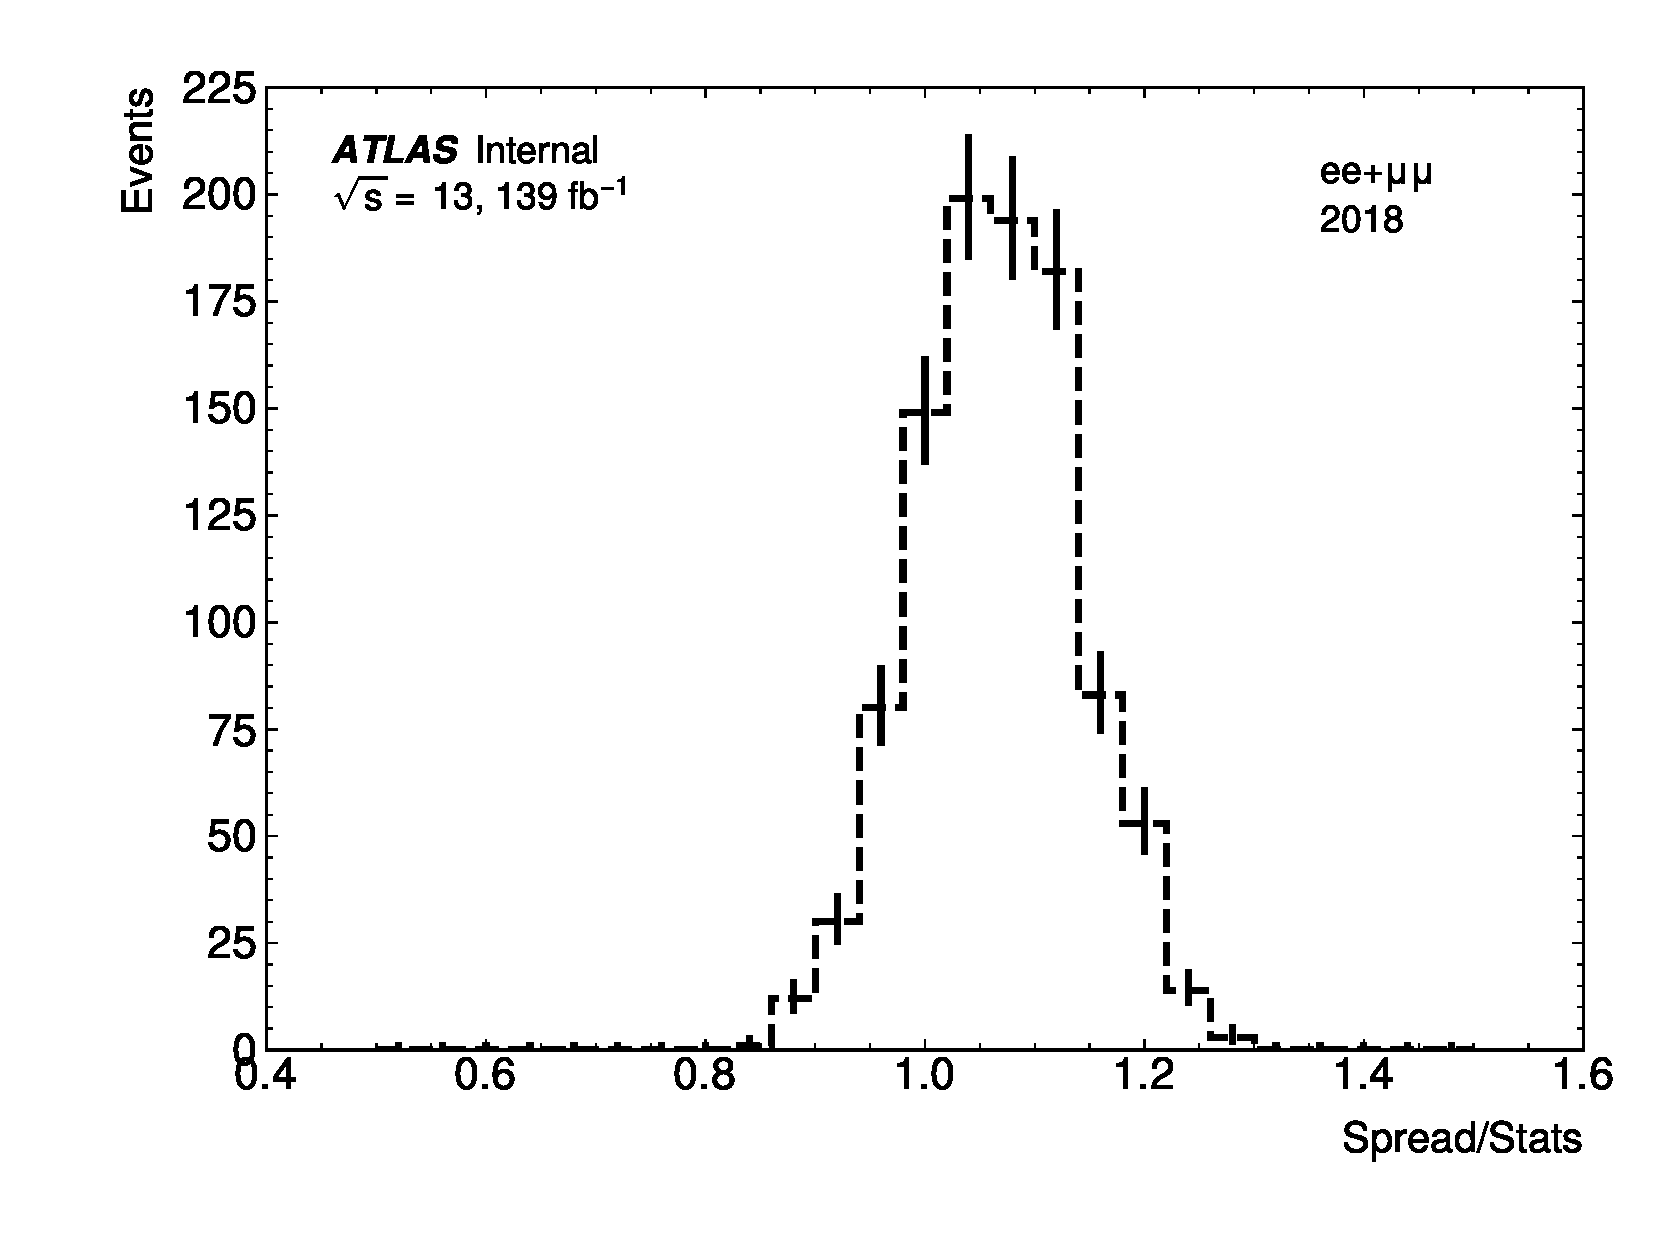
\includegraphics[width=0.45\textwidth]{figs/partially_unblinded_results/spread_stats_scrambled_data18_Ratio.pdf}
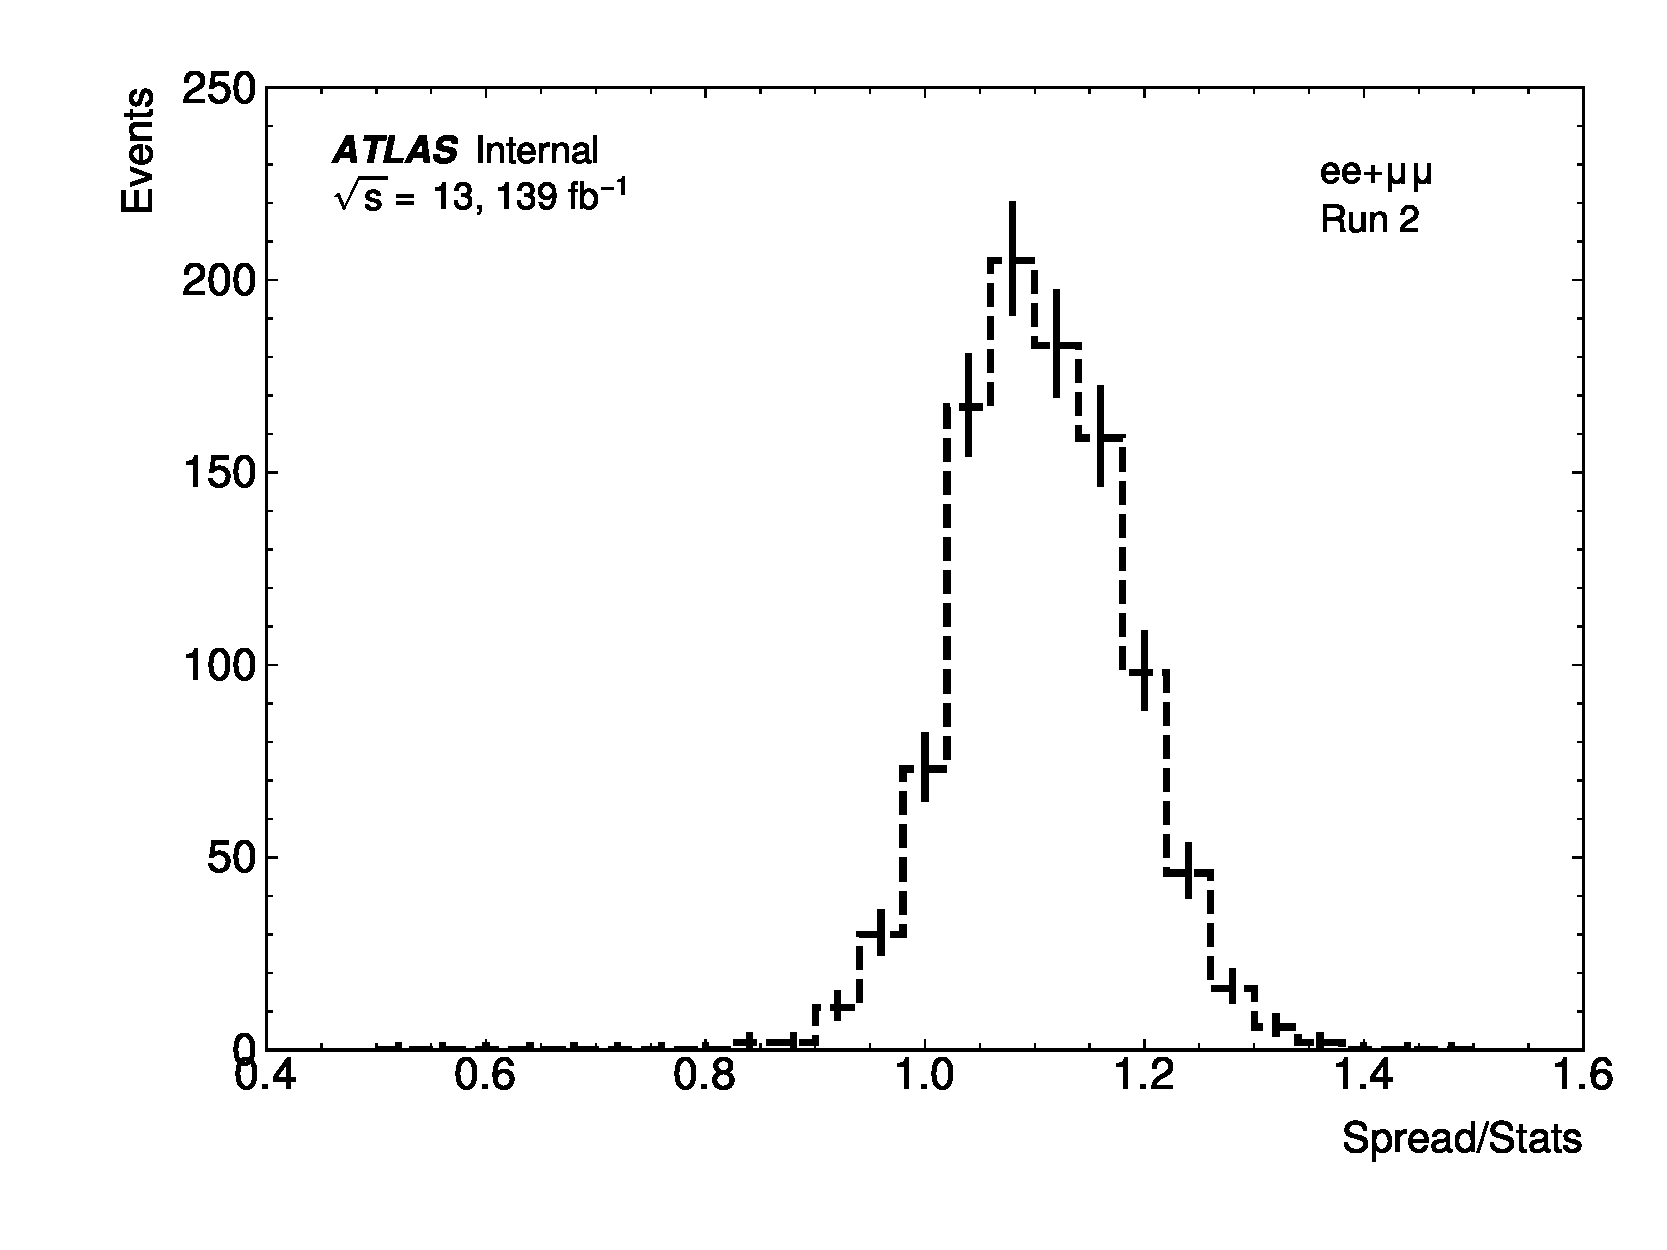
\includegraphics[width=0.45\textwidth]{figs/partially_unblinded_results/spread_stats_scrambled_full_Ratio.pdf}
\caption{Spreads VS average stats. Plots show average results of 1000 scrambled datasets. 
An average statistic is the average statistical uncertainty in each scrambled dataset, and the spread of a dataset is an average of absolute residual, e.g., $|1-data|4$. 
The 2015+2016 dataset(top left), the 2017 dataset (top right), the 2018 dataset(bottom left), and the Run 2 dataset (bottom right). The Run 2 dataset is the sum of all year's data. 
Spread is about 10-20\% larger in most of the scrambled datasets. This indicates there is a small systematic effect or the way we are calculating the ZC error in the double ratio. This could be the reason why the average values shifted from zero}
\label{fig:real_data_scrambled_Spreads_Stats}
\end{figure}


\subsubsection{Spurious signal uncertainty}

\begin{figure}[ht]
\centering

\includegraphics[width=0.45\textwidth]{figs/partially_unblinded_results/profile_chi2_shape_sys_du_XZ.pdf}
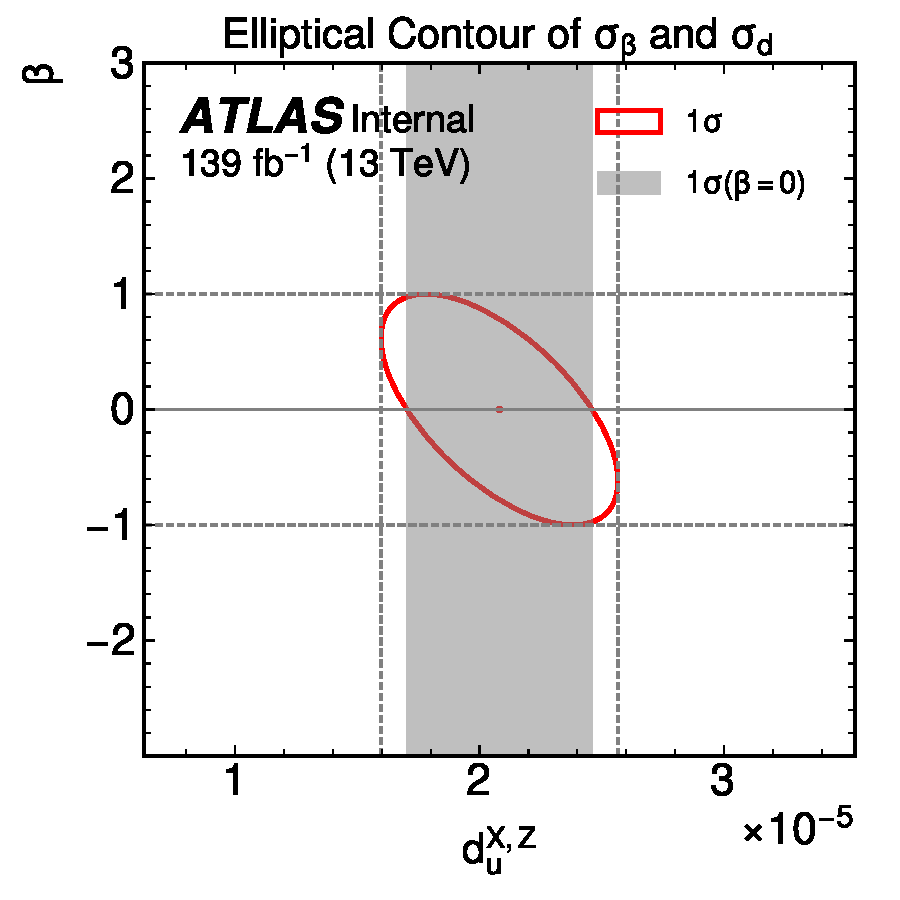
\includegraphics[width=0.45\textwidth]{figs/partially_unblinded_results/profile_chi2_shape_sys_du_XZ_sig0009.pdf}

\caption{Combined fit results of profiled $\chi^{2}$ fit, which includes the spurious signal uncertainty as a nuisance parameter $\beta$. The left plot is the result from one of the scrambled datasets. The right plot is a signal-injected toy dataset with strength $\sigma_{LIV}/\sigma_{SM}=0.0009$; the signal model is $d_{u}^{X,Z}$. 
The grey band is the 68\% uncertainty band without spurious signal. The fit uncertainty is 29(28 for the toy)\% larger when we add the spurious signal uncertainty to the fit.}
\label{fig:real_data_scrambled_Spurious_signal}
\end{figure}


\begin{figure}[ht]
\centering
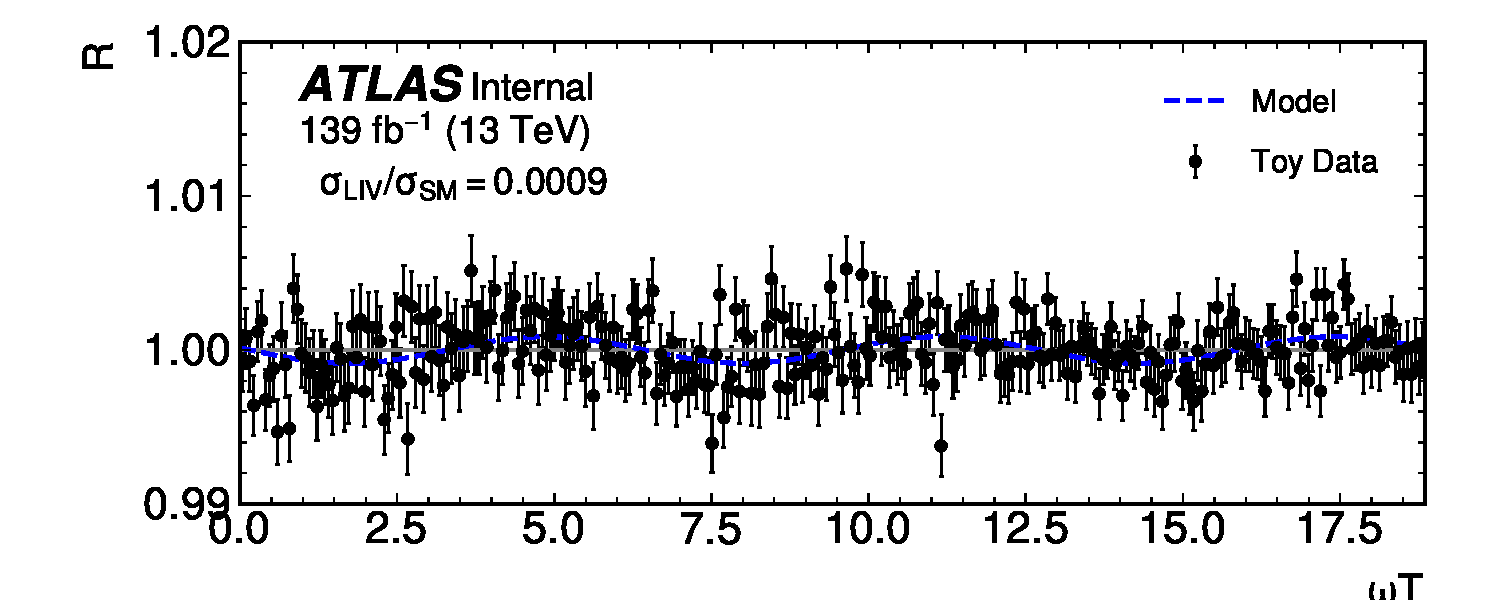
\includegraphics[width=0.90\textwidth]{figs/partially_unblinded_results/profile_chi2_toy_du_XZ_postfit_sig0009.pdf}

\caption{The signal-injected combined toy dataset with signal strength $\sigma_{LIV}/\sigma_{SM}=0.0009$ and  $d_{u}^{X,Z}$ model (post-fit). The blue line is the signal shape after the combined fit. The  error bars on the data points are statistical errors.}
\label{fig:real_data_scrambled_Spurious_signal}
\end{figure}






%%%%%%%%%%%%%%%%%%%%%%%%%%%%%%%%%%%%%%%%%%%%%%%%%%%%%%
%%%%%%%%%%%%%%%%%%%%%%%%%%%%%%%%%%%%%%%%%%%%%%%%%%%%%%
%%%%%%%%%%%%%%%%%%%%%%%%%%%%%%%%%%%%%%%%%%%%%%%%%%%%%%
\clearpage
\subsection{Partially unblinded data in deffirent periods}

\begin{table}
    \begin{center}
    \Rotatebox{90}{
    %%\resizebox{\textwidth}{!}{
    \begin{tabular}{| l| c| c| c| c|}
    \hline
     & 2015+2016 & 2017 & 2018  & Combined \\
     \hline
     $d_{\it u}^{\it X,Z}$  & -1.39e-05 $\pm$ 7.12e-06 & 6.46e-06 $\pm$ 6.58e-06 & 8.55e-06 $\pm$ 5.68e-06 & 1.74e-06 $\pm$ 3.58e-06\\
     \hline 
     $d_{\it u}^{\it Y,Z}$  & -6.42e-06 $\pm$ 6.79e-06 & 5.64e-06 $\pm$ 6.41e-06 & -2.04e-06 $\pm$ 5.81e-06 & -1.12e-06 $\pm$ 3.62e-06\\
     \hline 
     $d_{\it u}^{\it XY,XY}$  & -4.40e-08 $\pm$ 3.76e-06 & 7.80e-07 $\pm$ 3.36e-06 & -3.06e-06 $\pm$ 3.03e-06 & -1.18e-06 $\pm$ 1.91e-06\\
     \hline 
     $d_{\it u}^{\it X,Y}$  & 6.88e-07 $\pm$ 1.84e-06 & -1.75e-07 $\pm$ 1.70e-06 & -3.07e-09 $\pm$ 1.48e-06 & 1.50e-07 $\pm$ 9.86e-07\\
     \hline 
     $c_{\it u}^{\it X,Z}$  & -1.08e-05 $\pm$ 5.53e-06 & 5.02e-06 $\pm$ 5.11e-06 & 6.64e-06 $\pm$ 4.41e-06 & 1.35e-06 $\pm$ 2.78e-06\\
     \hline 
     $c_{\it u}^{\it Y,Z}$  & -4.99e-06 $\pm$ 5.28e-06 & 4.38e-06 $\pm$ 4.98e-06 & -1.58e-06 $\pm$ 4.51e-06 & -8.69e-07 $\pm$ 2.81e-06\\
     \hline 
     $c_{\it u}^{\it XY,XY}$  & -3.42e-08 $\pm$ 2.92e-06 & 6.06e-07 $\pm$ 2.61e-06 & -2.38e-06 $\pm$ 2.35e-06 & -9.18e-07 $\pm$ 1.49e-06\\
     \hline 
     $c_{\it u}^{\it X,Y}$  & 5.34e-07 $\pm$ 1.43e-06 & -1.36e-07 $\pm$ 1.32e-06 & -2.39e-09 $\pm$ 1.15e-06 & 1.16e-07 $\pm$ 7.66e-07\\
     \hline 
     $c_{\it d}^{\it X,Z}$  & -4.80e-04 $\pm$ 2.46e-04 & 2.24e-04 $\pm$ 2.28e-04 & 2.96e-04 $\pm$ 1.97e-04 & 6.03e-05 $\pm$ 1.24e-04\\
     \hline 
     $c_{\it d}^{\it Y,Z}$  & -2.22e-04 $\pm$ 2.35e-04 & 1.95e-04 $\pm$ 2.22e-04 & -7.05e-05 $\pm$ 2.01e-04 & -3.87e-05 $\pm$ 1.25e-04\\
     \hline 
     $c_{\it d}^{\it XY,XY}$  & -1.52e-06 $\pm$ 1.30e-04 & 2.70e-05 $\pm$ 1.16e-04 & -1.06e-04 $\pm$ 1.05e-04 & -4.09e-05 $\pm$ 6.62e-05\\
     \hline 
     $c_{\it d}^{\it X,Y}$  & 2.38e-05 $\pm$ 6.36e-05 & -6.05e-06 $\pm$ 5.90e-05 & -1.07e-07 $\pm$ 5.14e-05 & 5.17e-06 $\pm$ 3.41e-05\\
     \hline 
     \hline
    \end{tabular}
    }%
    \end{center}
    \caption{ Results fo scrampled dataset in 1 hour period;
     results are obtained from combinded Run 2 fit.
    \label{table:scrambled_1hour}}
\end{table}
    

\begin{table}
        \begin{center}
        \Rotatebox{90}{
        %%\resizebox{\textwidth}{!}{
        \begin{tabular}{| l| c| c| c| c|}
        \hline
         & 2015+2016 & 2017 & 2018  & Combined \\
         \hline
         $d_{\it u}^{\it X,Z}$  & 1.18e-06 $\pm$ 6.78e-06 & -8.37e-06 $\pm$ 6.71e-06 & -4.42e-06 $\pm$ 5.73e-06 & -4.16e-06 $\pm$ 3.72e-06\\
         \hline 
         $d_{\it u}^{\it Y,Z}$  & -6.04e-06 $\pm$ 6.89e-06 & 4.05e-06 $\pm$ 6.50e-06 & -6.26e-06 $\pm$ 5.90e-06 & -3.25e-06 $\pm$ 3.70e-06\\
         \hline 
         $d_{\it u}^{\it XY,XY}$  & -3.65e-07 $\pm$ 3.74e-06 & -3.97e-06 $\pm$ 3.30e-06 & 2.09e-07 $\pm$ 2.96e-06 & -1.41e-06 $\pm$ 1.83e-06\\
         \hline 
         $d_{\it u}^{\it X,Y}$  & -6.08e-07 $\pm$ 1.87e-06 & -2.89e-06 $\pm$ 1.66e-06 & 1.22e-06 $\pm$ 1.42e-06 & -5.49e-07 $\pm$ 9.44e-07\\
         \hline 
         $c_{\it u}^{\it X,Z}$  & 9.19e-07 $\pm$ 5.26e-06 & -6.50e-06 $\pm$ 5.21e-06 & -3.43e-06 $\pm$ 4.45e-06 & -3.23e-06 $\pm$ 2.89e-06\\
         \hline 
         $c_{\it u}^{\it Y,Z}$  & -4.69e-06 $\pm$ 5.36e-06 & 3.15e-06 $\pm$ 5.05e-06 & -4.87e-06 $\pm$ 4.58e-06 & -2.52e-06 $\pm$ 2.87e-06\\
         \hline 
         $c_{\it u}^{\it XY,XY}$  & -2.84e-07 $\pm$ 2.90e-06 & -3.08e-06 $\pm$ 2.57e-06 & 1.62e-07 $\pm$ 2.30e-06 & -1.09e-06 $\pm$ 1.42e-06\\
         \hline 
         $c_{\it u}^{\it X,Y}$  & -4.72e-07 $\pm$ 1.45e-06 & -2.24e-06 $\pm$ 1.29e-06 & 9.45e-07 $\pm$ 1.11e-06 & -4.27e-07 $\pm$ 7.33e-07\\
         \hline 
         $c_{\it d}^{\it X,Z}$  & 4.09e-05 $\pm$ 2.34e-04 & -2.89e-04 $\pm$ 2.32e-04 & -1.53e-04 $\pm$ 1.98e-04 & -1.44e-04 $\pm$ 1.29e-04\\
         \hline 
         $c_{\it d}^{\it Y,Z}$  & -2.09e-04 $\pm$ 2.39e-04 & 1.40e-04 $\pm$ 2.25e-04 & -2.17e-04 $\pm$ 2.04e-04 & -1.12e-04 $\pm$ 1.28e-04\\
         \hline 
         $c_{\it d}^{\it XY,XY}$  & -1.26e-05 $\pm$ 1.29e-04 & -1.37e-04 $\pm$ 1.14e-04 & 7.23e-06 $\pm$ 1.02e-04 & -4.86e-05 $\pm$ 6.33e-05\\
         \hline 
         $c_{\it d}^{\it X,Y}$  & -2.10e-05 $\pm$ 6.47e-05 & -9.99e-05 $\pm$ 5.74e-05 & 4.21e-05 $\pm$ 4.92e-05 & -1.90e-05 $\pm$ 3.27e-05\\
         \hline 
         \hline
        \end{tabular}
        }%
        \end{center}
        \caption{ Results fo scrampled dataset in 6.87 hours period;
        results are obtained from combinded Run 2 fit.
       \label{table:scrambled_6_87hour}}
\end{table}


\begin{table}
            \begin{center}
            \Rotatebox{90}{
            %%\resizebox{\textwidth}{!}{
            \begin{tabular}{| l| c| c| c| c|}
            \hline
             & 2015+2016 & 2017 & 2018  & Combined \\
             \hline
             $d_{\it u}^{\it X,Z}$  & 8.10e-06 $\pm$ 7.12e-06 & -1.58e-06 $\pm$ 6.43e-06 & 1.94e-07 $\pm$ 5.71e-06 & 1.75e-06 $\pm$ 3.71e-06\\
             \hline 
             $d_{\it u}^{\it Y,Z}$  & -1.93e-06 $\pm$ 7.00e-06 & 1.68e-06 $\pm$ 6.69e-06 & 1.10e-05 $\pm$ 6.07e-06 & 4.24e-06 $\pm$ 3.74e-06\\
             \hline 
             $d_{\it u}^{\it XY,XY}$  & -1.13e-06 $\pm$ 3.71e-06 & 1.80e-06 $\pm$ 3.31e-06 & 8.12e-06 $\pm$ 2.86e-06 & 3.46e-06 $\pm$ 1.95e-06\\
             \hline 
             $d_{\it u}^{\it X,Y}$  & 6.74e-07 $\pm$ 1.84e-06 & 1.94e-06 $\pm$ 1.63e-06 & -2.57e-07 $\pm$ 1.43e-06 & 7.05e-07 $\pm$ 9.49e-07\\
             \hline 
             $c_{\it u}^{\it X,Z}$  & 6.30e-06 $\pm$ 5.53e-06 & -1.23e-06 $\pm$ 5.00e-06 & 1.51e-07 $\pm$ 4.44e-06 & 1.36e-06 $\pm$ 2.88e-06\\
             \hline 
             $c_{\it u}^{\it Y,Z}$  & -1.50e-06 $\pm$ 5.44e-06 & 1.30e-06 $\pm$ 5.20e-06 & 8.53e-06 $\pm$ 4.72e-06 & 3.29e-06 $\pm$ 2.91e-06\\
             \hline 
             $c_{\it u}^{\it XY,XY}$  & -8.81e-07 $\pm$ 2.88e-06 & 1.40e-06 $\pm$ 2.58e-06 & 6.31e-06 $\pm$ 2.22e-06 & 2.69e-06 $\pm$ 1.52e-06\\
             \hline 
             $c_{\it u}^{\it X,Y}$  & 5.24e-07 $\pm$ 1.43e-06 & 1.51e-06 $\pm$ 1.27e-06 & -2.00e-07 $\pm$ 1.11e-06 & 5.48e-07 $\pm$ 7.38e-07\\
             \hline 
             $c_{\it d}^{\it X,Z}$  & 2.80e-04 $\pm$ 2.46e-04 & -5.46e-05 $\pm$ 2.22e-04 & 6.71e-06 $\pm$ 1.98e-04 & 6.06e-05 $\pm$ 1.28e-04\\
             \hline 
             $c_{\it d}^{\it Y,Z}$  & -6.69e-05 $\pm$ 2.42e-04 & 5.80e-05 $\pm$ 2.32e-04 & 3.80e-04 $\pm$ 2.10e-04 & 1.47e-04 $\pm$ 1.29e-04\\
             \hline 
             $c_{\it d}^{\it XY,XY}$  & -3.92e-05 $\pm$ 1.28e-04 & 6.23e-05 $\pm$ 1.15e-04 & 2.81e-04 $\pm$ 9.90e-05 & 1.20e-04 $\pm$ 6.76e-05\\
             \hline 
             $c_{\it d}^{\it X,Y}$  & 2.33e-05 $\pm$ 6.38e-05 & 6.72e-05 $\pm$ 5.66e-05 & -8.90e-06 $\pm$ 4.95e-05 & 2.44e-05 $\pm$ 3.28e-05\\
             \hline 
             \hline
            \end{tabular}
            }%
            \end{center}
            \caption{  Results fo scrampled dataset in 7 hours period;
            results are obtained from combinded Run 2 fit.
           \label{table:scrambled_7hour}}
\end{table}


\begin{table}
                \begin{center}
                \Rotatebox{90}{
                %%\resizebox{\textwidth}{!}{
                \begin{tabular}{| l| c| c| c| c|}
                \hline
                 & 2015+2016 & 2017 & 2018  & Combined \\
                 \hline
                 $d_{\it u}^{\it X,Z}$  & -8.00e-06 $\pm$ 7.06e-06 & -6.57e-06 $\pm$ 6.28e-06 & -6.15e-06 $\pm$ 5.90e-06 & -6.82e-06 $\pm$ 3.67e-06\\
                 \hline 
                 $d_{\it u}^{\it Y,Z}$  & -7.00e-06 $\pm$ 7.35e-06 & 5.72e-06 $\pm$ 6.72e-06 & 5.02e-06 $\pm$ 5.87e-06 & 1.66e-06 $\pm$ 3.81e-06\\
                 \hline 
                 $d_{\it u}^{\it XY,XY}$  & -4.21e-06 $\pm$ 3.84e-06 & 5.75e-06 $\pm$ 3.27e-06 & 2.04e-06 $\pm$ 3.01e-06 & 1.36e-06 $\pm$ 1.90e-06\\
                 \hline 
                 $d_{\it u}^{\it X,Y}$  & -5.23e-07 $\pm$ 1.80e-06 & -2.51e-07 $\pm$ 1.62e-06 & 7.32e-07 $\pm$ 1.41e-06 & 9.90e-08 $\pm$ 9.29e-07\\
                 \hline 
                 $c_{\it u}^{\it X,Z}$  & -6.21e-06 $\pm$ 5.48e-06 & -5.11e-06 $\pm$ 4.88e-06 & -4.78e-06 $\pm$ 4.58e-06 & -5.30e-06 $\pm$ 2.85e-06\\
                 \hline 
                 $c_{\it u}^{\it Y,Z}$  & -5.44e-06 $\pm$ 5.71e-06 & 4.44e-06 $\pm$ 5.22e-06 & 3.90e-06 $\pm$ 4.56e-06 & 1.29e-06 $\pm$ 2.96e-06\\
                 \hline 
                 $c_{\it u}^{\it XY,XY}$  & -3.27e-06 $\pm$ 2.99e-06 & 4.47e-06 $\pm$ 2.54e-06 & 1.58e-06 $\pm$ 2.34e-06 & 1.06e-06 $\pm$ 1.48e-06\\
                 \hline 
                 $c_{\it u}^{\it X,Y}$  & -4.07e-07 $\pm$ 1.40e-06 & -1.95e-07 $\pm$ 1.26e-06 & 5.69e-07 $\pm$ 1.10e-06 & 7.69e-08 $\pm$ 7.22e-07\\
                 \hline 
                 $c_{\it d}^{\it X,Z}$  & -2.77e-04 $\pm$ 2.44e-04 & -2.27e-04 $\pm$ 2.17e-04 & -2.13e-04 $\pm$ 2.04e-04 & -2.36e-04 $\pm$ 1.27e-04\\
                 \hline 
                 $c_{\it d}^{\it Y,Z}$  & -2.42e-04 $\pm$ 2.54e-04 & 1.98e-04 $\pm$ 2.33e-04 & 1.74e-04 $\pm$ 2.03e-04 & 5.73e-05 $\pm$ 1.32e-04\\
                 \hline 
                 $c_{\it d}^{\it XY,XY}$  & -1.46e-04 $\pm$ 1.33e-04 & 1.99e-04 $\pm$ 1.13e-04 & 7.05e-05 $\pm$ 1.04e-04 & 4.70e-05 $\pm$ 6.59e-05\\
                 \hline 
                 $c_{\it d}^{\it X,Y}$  & -1.81e-05 $\pm$ 6.22e-05 & -8.68e-06 $\pm$ 5.62e-05 & 2.53e-05 $\pm$ 4.89e-05 & 3.42e-06 $\pm$ 3.21e-05\\
                 \hline 
                 \hline
                \end{tabular}
                }%
                \end{center}
                \caption{ Results fo scrampled dataset in 7.13 hours period;
                results are obtained from combinded Run 2 fit.
               \label{table:scrambled_7_13hour}}
\end{table}
                
                
\begin{table}
                    \begin{center}
                    \Rotatebox{90}{
                    %%\resizebox{\textwidth}{!}{
                    \begin{tabular}{| l| c| c| c| c|}
                    \hline
                     & 2015+2016 & 2017 & 2018  & Combined \\
                     \hline
                     & 2015+2016 & 2017 & 2018  & Combined \\
                    \hline
                    $d_{\it u}^{\it X,Z}$  & -8.76e-06 $\pm$ 7.24e-06 & 1.11e-05 $\pm$ 6.49e-06 & -2.64e-06 $\pm$ 5.58e-06 & 4.22e-08 $\pm$ 3.58e-06\\
                    \hline 
                    $d_{\it u}^{\it Y,Z}$  & -4.61e-06 $\pm$ 6.96e-06 & -1.05e-05 $\pm$ 6.51e-06 & 7.20e-06 $\pm$ 5.76e-06 & -1.85e-06 $\pm$ 3.65e-06\\
                    \hline 
                    $d_{\it u}^{\it XY,XY}$  & -1.46e-06 $\pm$ 3.76e-06 & 4.86e-06 $\pm$ 3.27e-06 & -1.96e-06 $\pm$ 2.85e-06 & 1.88e-07 $\pm$ 1.86e-06\\
                    \hline 
                    $d_{\it u}^{\it X,Y}$  & -2.54e-07 $\pm$ 1.86e-06 & -1.27e-06 $\pm$ 1.61e-06 & -5.87e-07 $\pm$ 1.49e-06 & -6.93e-07 $\pm$ 9.24e-07\\
                    \hline 
                    $c_{\it u}^{\it X,Z}$  & -6.81e-06 $\pm$ 5.63e-06 & 8.62e-06 $\pm$ 5.05e-06 & -2.05e-06 $\pm$ 4.33e-06 & 3.28e-08 $\pm$ 2.78e-06\\
                    \hline 
                    $c_{\it u}^{\it Y,Z}$  & -3.58e-06 $\pm$ 5.41e-06 & -8.13e-06 $\pm$ 5.06e-06 & 5.60e-06 $\pm$ 4.47e-06 & -1.44e-06 $\pm$ 2.84e-06\\
                    \hline 
                    $c_{\it u}^{\it XY,XY}$  & -1.14e-06 $\pm$ 2.92e-06 & 3.78e-06 $\pm$ 2.54e-06 & -1.53e-06 $\pm$ 2.21e-06 & 1.46e-07 $\pm$ 1.44e-06\\
                    \hline 
                    $c_{\it u}^{\it X,Y}$  & -1.98e-07 $\pm$ 1.44e-06 & -9.90e-07 $\pm$ 1.25e-06 & -4.56e-07 $\pm$ 1.15e-06 & -5.39e-07 $\pm$ 7.18e-07\\
                    \hline 
                    $c_{\it d}^{\it X,Z}$  & -3.03e-04 $\pm$ 2.51e-04 & 3.84e-04 $\pm$ 2.25e-04 & -9.12e-05 $\pm$ 1.93e-04 & 1.46e-06 $\pm$ 1.24e-04\\
                    \hline 
                    $c_{\it d}^{\it Y,Z}$  & -1.60e-04 $\pm$ 2.41e-04 & -3.62e-04 $\pm$ 2.25e-04 & 2.49e-04 $\pm$ 1.99e-04 & -6.39e-05 $\pm$ 1.26e-04\\
                    \hline 
                    $c_{\it d}^{\it XY,XY}$  & -5.07e-05 $\pm$ 1.30e-04 & 1.68e-04 $\pm$ 1.13e-04 & -6.79e-05 $\pm$ 9.84e-05 & 6.49e-06 $\pm$ 6.43e-05\\
                    \hline 
                    $c_{\it d}^{\it X,Y}$  & -8.80e-06 $\pm$ 6.42e-05 & -4.41e-05 $\pm$ 5.56e-05 & -2.03e-05 $\pm$ 5.14e-05 & -2.40e-05 $\pm$ 3.20e-05\\
                    \hline 
                    \hline
                    \end{tabular}
                    }%
                    \end{center}
                    \caption{ Results fo scrampled dataset in 24 hours period;
                    results are obtained from combinded Run 2 fit.
                   \label{table:scrambled_24hour}}
\end{table}
                    
                    
\begin{table}
                        \begin{center}
                        \Rotatebox{90}{
                        %%\resizebox{\textwidth}{!}{
                        \begin{tabular}{| l| c| c| c| c|}
                        \hline
                         & 2015+2016 & 2017 & 2018  & Combined \\
                        \hline
                        $d_{\it u}^{\it X,Z}$  & 7.35e-06 $\pm$ 7.32e-06 & -7.07e-06 $\pm$ 6.61e-06 & -6.50e-06 $\pm$ 5.70e-06 & -2.99e-06 $\pm$ 3.62e-06\\
                        \hline 
                        $d_{\it u}^{\it Y,Z}$  & -4.18e-07 $\pm$ 7.22e-06 & 7.34e-06 $\pm$ 6.53e-06 & -1.08e-05 $\pm$ 5.82e-06 & -2.50e-06 $\pm$ 3.59e-06\\
                        \hline 
                        $d_{\it u}^{\it XY,XY}$  & -6.28e-07 $\pm$ 3.70e-06 & -1.91e-06 $\pm$ 3.36e-06 & 1.60e-06 $\pm$ 2.90e-06 & -2.39e-07 $\pm$ 1.89e-06\\
                        \hline 
                        $d_{\it u}^{\it X,Y}$  & -1.28e-06 $\pm$ 1.86e-06 & 5.44e-07 $\pm$ 1.66e-06 & 7.14e-07 $\pm$ 1.46e-06 & 1.41e-07 $\pm$ 9.40e-07\\
                        \hline 
                        $c_{\it u}^{\it X,Z}$  & 5.71e-06 $\pm$ 5.69e-06 & -5.49e-06 $\pm$ 5.13e-06 & -5.05e-06 $\pm$ 4.43e-06 & -2.32e-06 $\pm$ 2.81e-06\\
                        \hline 
                        $c_{\it u}^{\it Y,Z}$  & -3.25e-07 $\pm$ 5.61e-06 & 5.70e-06 $\pm$ 5.07e-06 & -8.39e-06 $\pm$ 4.52e-06 & -1.94e-06 $\pm$ 2.79e-06\\
                        \hline 
                        $c_{\it u}^{\it XY,XY}$  & -4.88e-07 $\pm$ 2.88e-06 & -1.48e-06 $\pm$ 2.61e-06 & 1.25e-06 $\pm$ 2.26e-06 & -1.86e-07 $\pm$ 1.47e-06\\
                        \hline 
                        $c_{\it u}^{\it X,Y}$  & -9.96e-07 $\pm$ 1.45e-06 & 4.22e-07 $\pm$ 1.29e-06 & 5.55e-07 $\pm$ 1.14e-06 & 1.09e-07 $\pm$ 7.31e-07\\
                        \hline 
                        $c_{\it d}^{\it X,Z}$  & 2.54e-04 $\pm$ 2.53e-04 & -2.45e-04 $\pm$ 2.29e-04 & -2.25e-04 $\pm$ 1.97e-04 & -1.03e-04 $\pm$ 1.25e-04\\
                        \hline 
                        $c_{\it d}^{\it Y,Z}$  & -1.45e-05 $\pm$ 2.50e-04 & 2.54e-04 $\pm$ 2.26e-04 & -3.73e-04 $\pm$ 2.01e-04 & -8.66e-05 $\pm$ 1.24e-04\\
                        \hline 
                        $c_{\it d}^{\it XY,XY}$  & -2.17e-05 $\pm$ 1.28e-04 & -6.60e-05 $\pm$ 1.16e-04 & 5.55e-05 $\pm$ 1.00e-04 & -8.27e-06 $\pm$ 6.54e-05\\
                        \hline 
                        $c_{\it d}^{\it X,Y}$  & -4.43e-05 $\pm$ 6.45e-05 & 1.88e-05 $\pm$ 5.76e-05 & 2.47e-05 $\pm$ 5.06e-05 & 4.86e-06 $\pm$ 3.25e-05\\
                        \hline 
                        \hline
                        \end{tabular}
                        }%
                        \end{center}
                        \caption{ Results fo scrampled dataset in sidereal hours period;
                        results are obtained from combinded Run 2 fit.
                       \label{table:scrambled_sidereal}}
\end{table}
                        
                        
            
        
        